
\section{Evaluation}
\label{sec5} 
We evaluate our work through two sets of evaluations: first, in an isolated setting as a standalone attention layer with causal mask applied, and second, in an end-to-end setting where we train an LLM. We refer to our implementation as `Our LA`, and compare our results with Gated LA~\cite{yang2023gated} (the state-of-the-art LA implementation), Speculative Decoding (Spec. Dec.) LA~\cite{you2024linear}, and baseline LA where we use the default Pytorch operations. We also compare with efficient I/O aware implementation of Regular Attention, FlashAttention-2~\cite{dao2024flashattention}.

\begin{figure*}[!h]
\minipage{0.499\linewidth} \begin{centering}
\hspace{25pt}\textbf{FP Time vs Sequence Length ($N$)}\par\medskip
  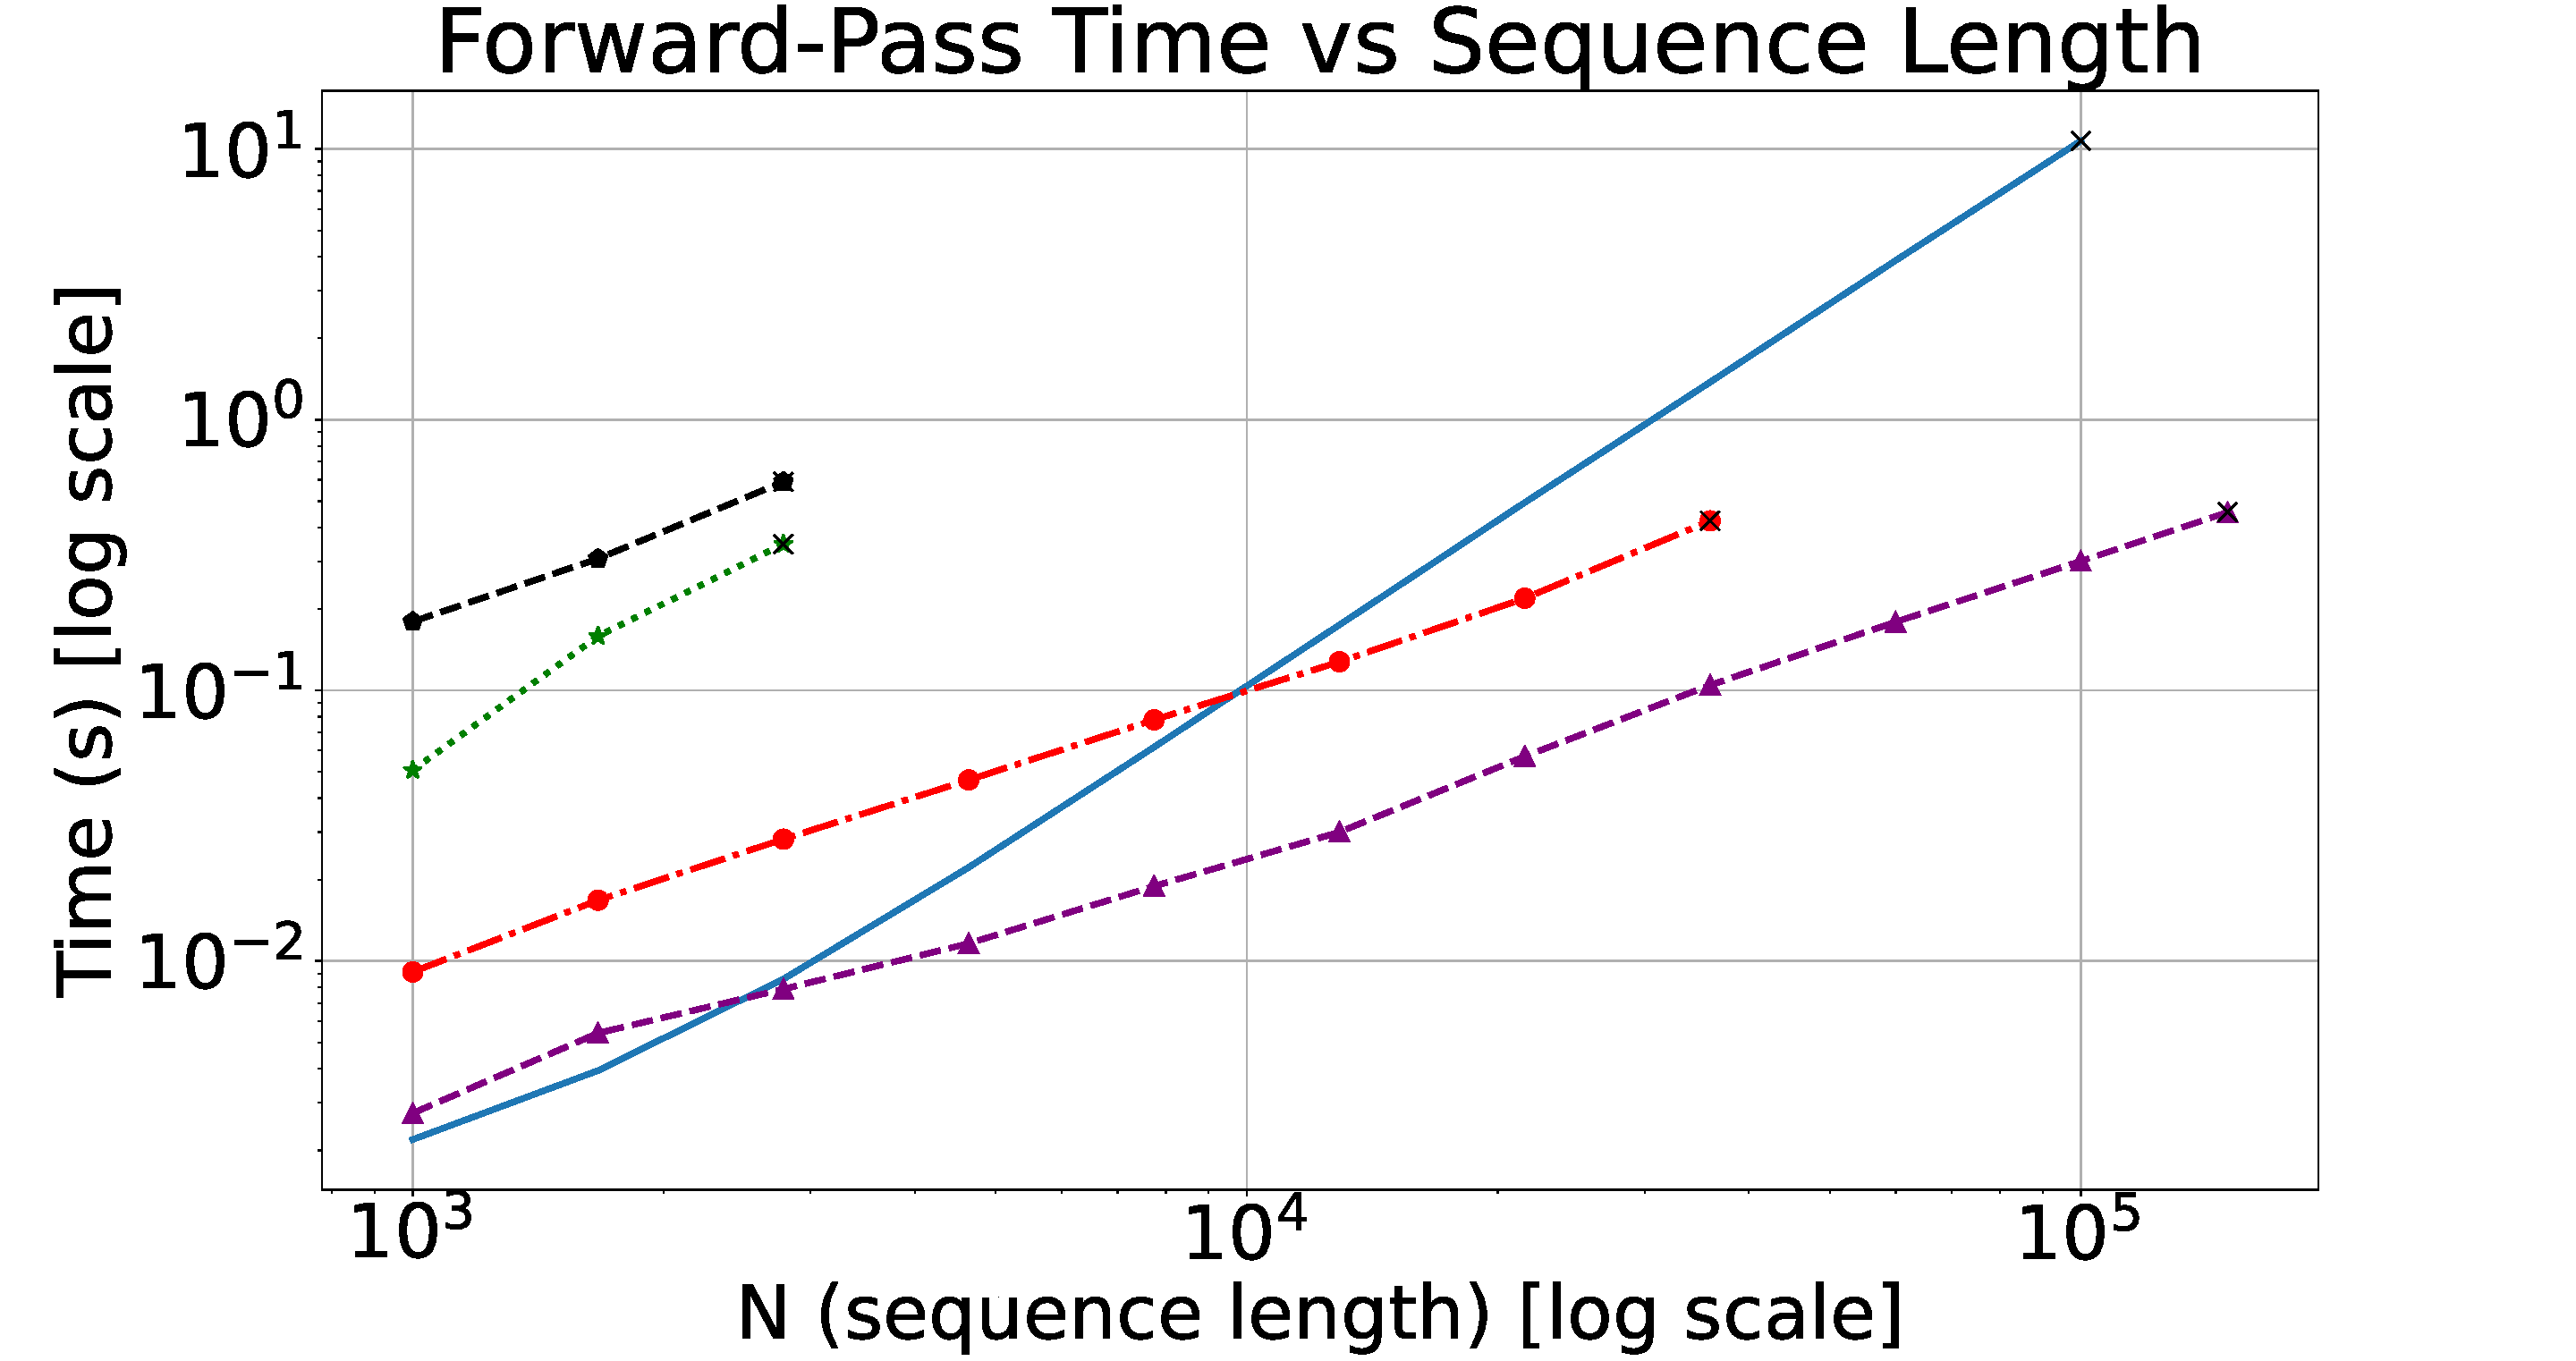
\includegraphics[width=\linewidth, trim=0mm 0mm 35mm 17mm, clip=true]{images/fp_tvn.pdf}
  \end{centering} \endminipage
\minipage{0.499\linewidth} \begin{centering}
\hspace{25pt}\textbf{FP Memory vs Sequence Length ($N$)}\par\medskip
  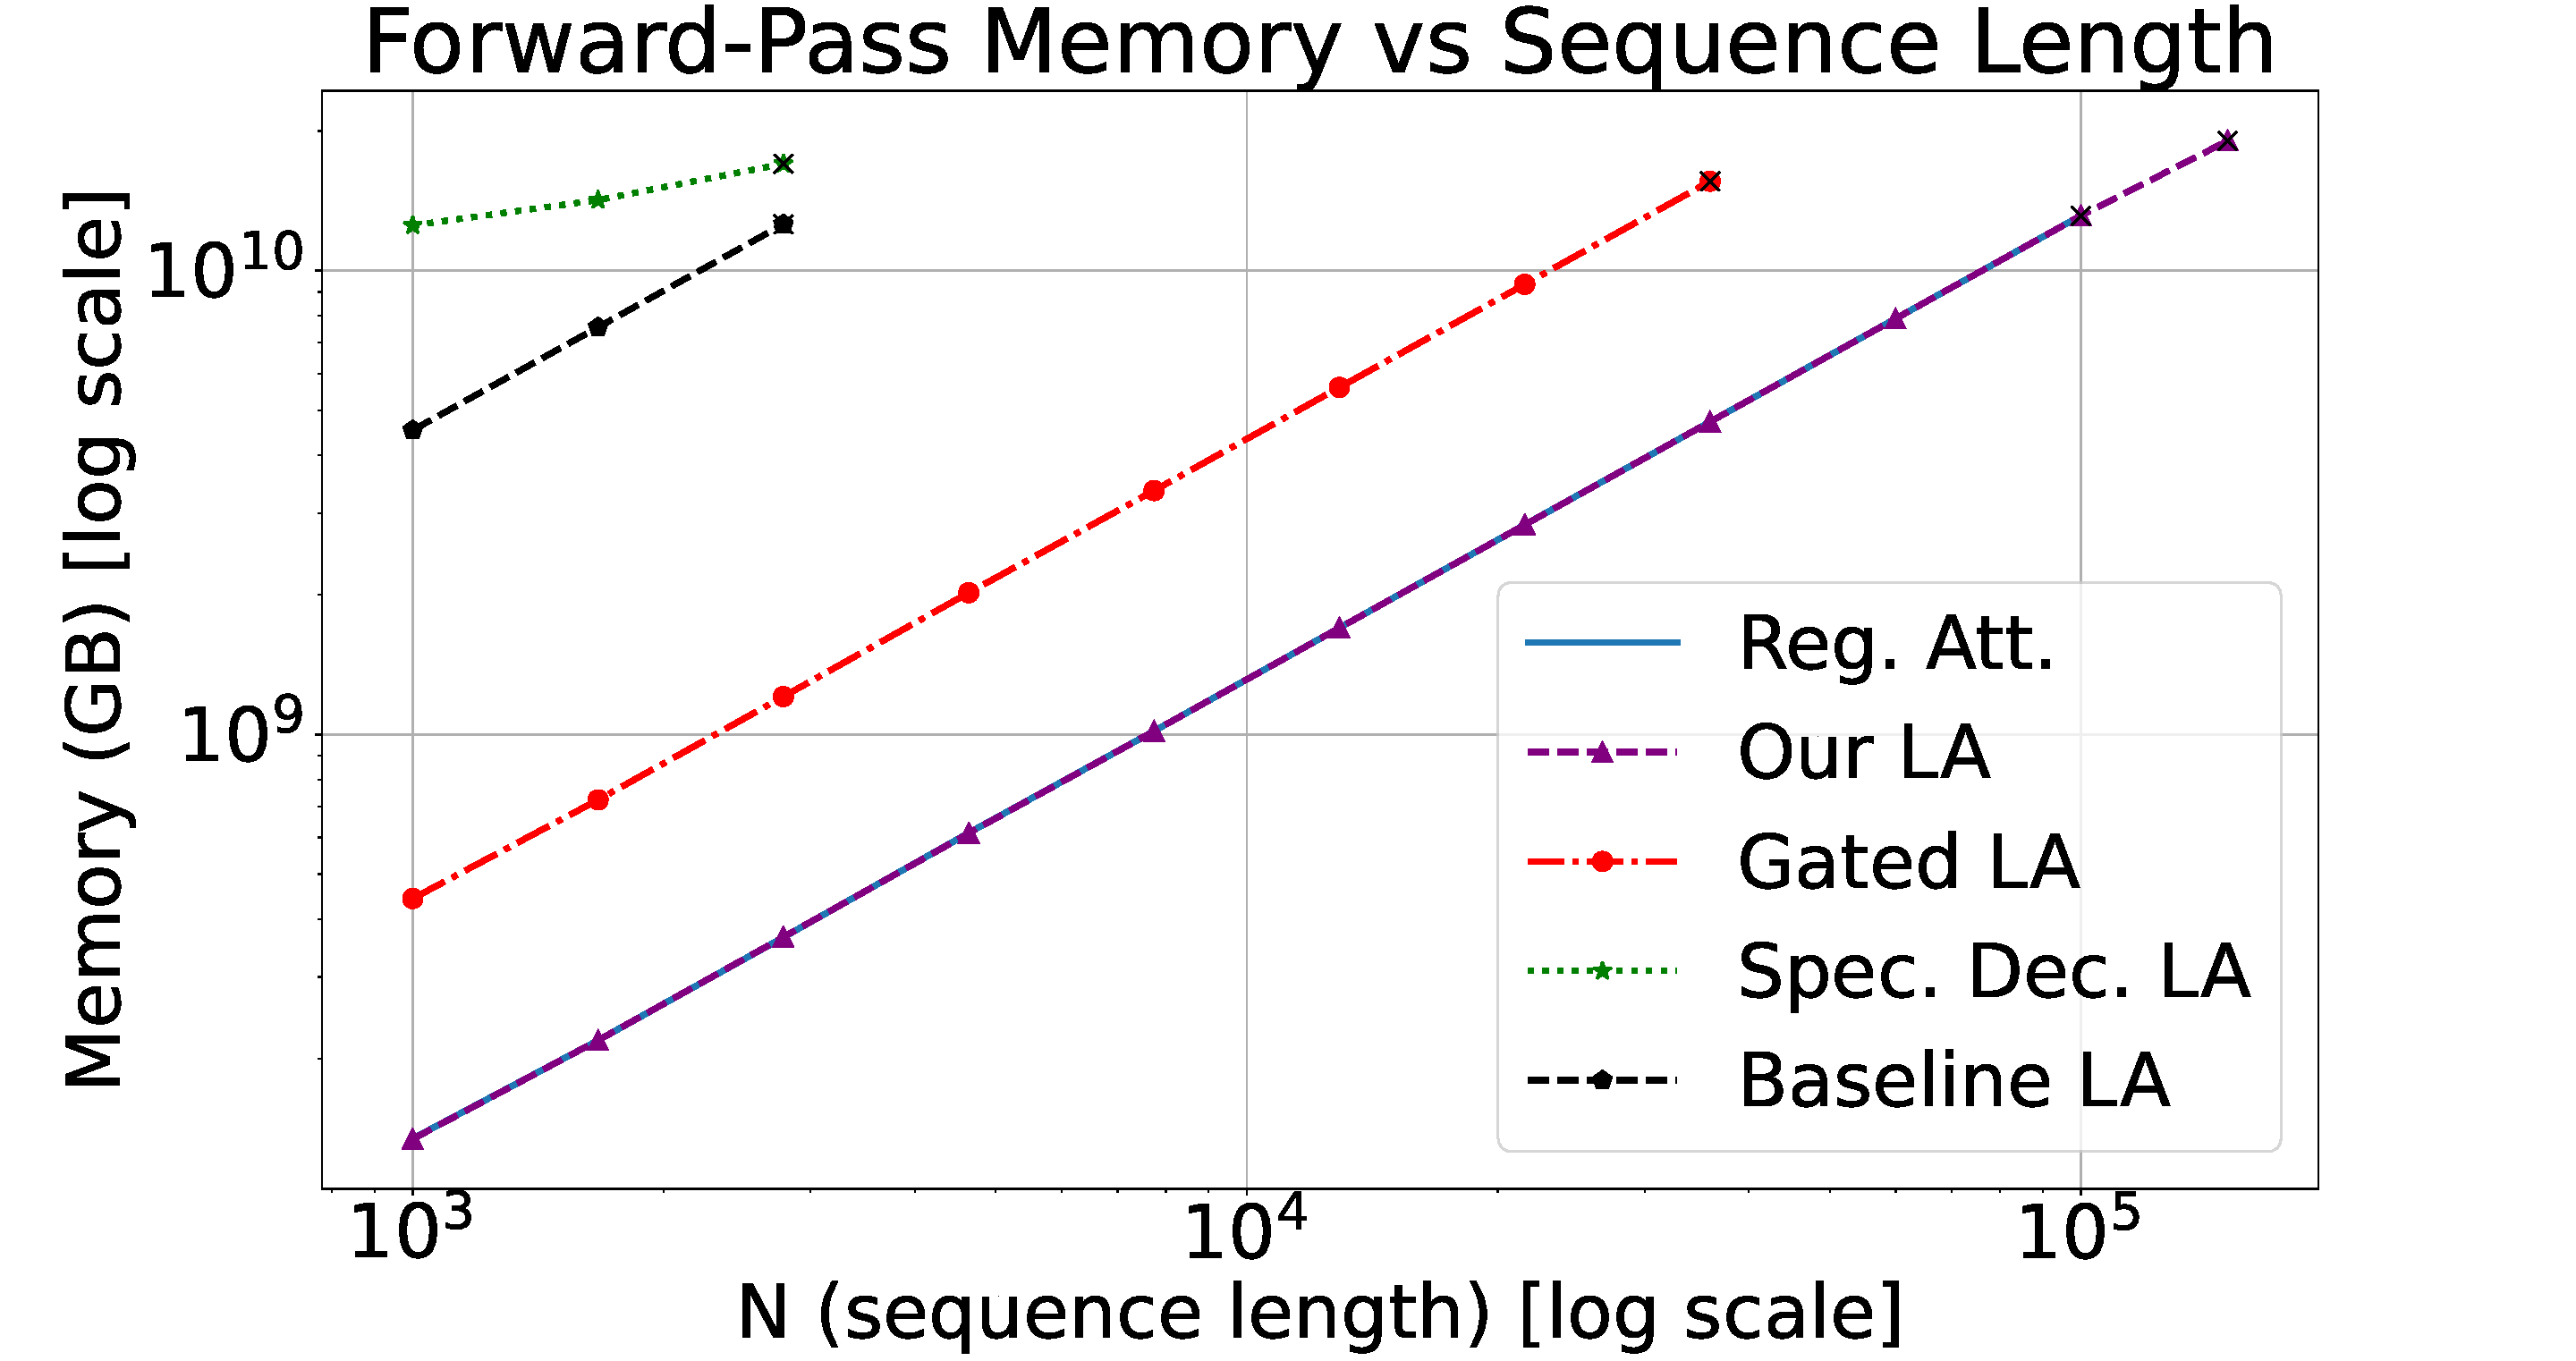
\includegraphics[width=\linewidth, trim=0mm 0mm 35mm 17mm, clip=true]{images/fp_mvn.pdf}
  \end{centering} \endminipage\hfill
% \vspace{20pt}
\minipage{0.499\linewidth} \begin{centering}
\hspace{25pt}\textbf{FP Time vs Dimension Per Head ($D$)}\par\medskip
  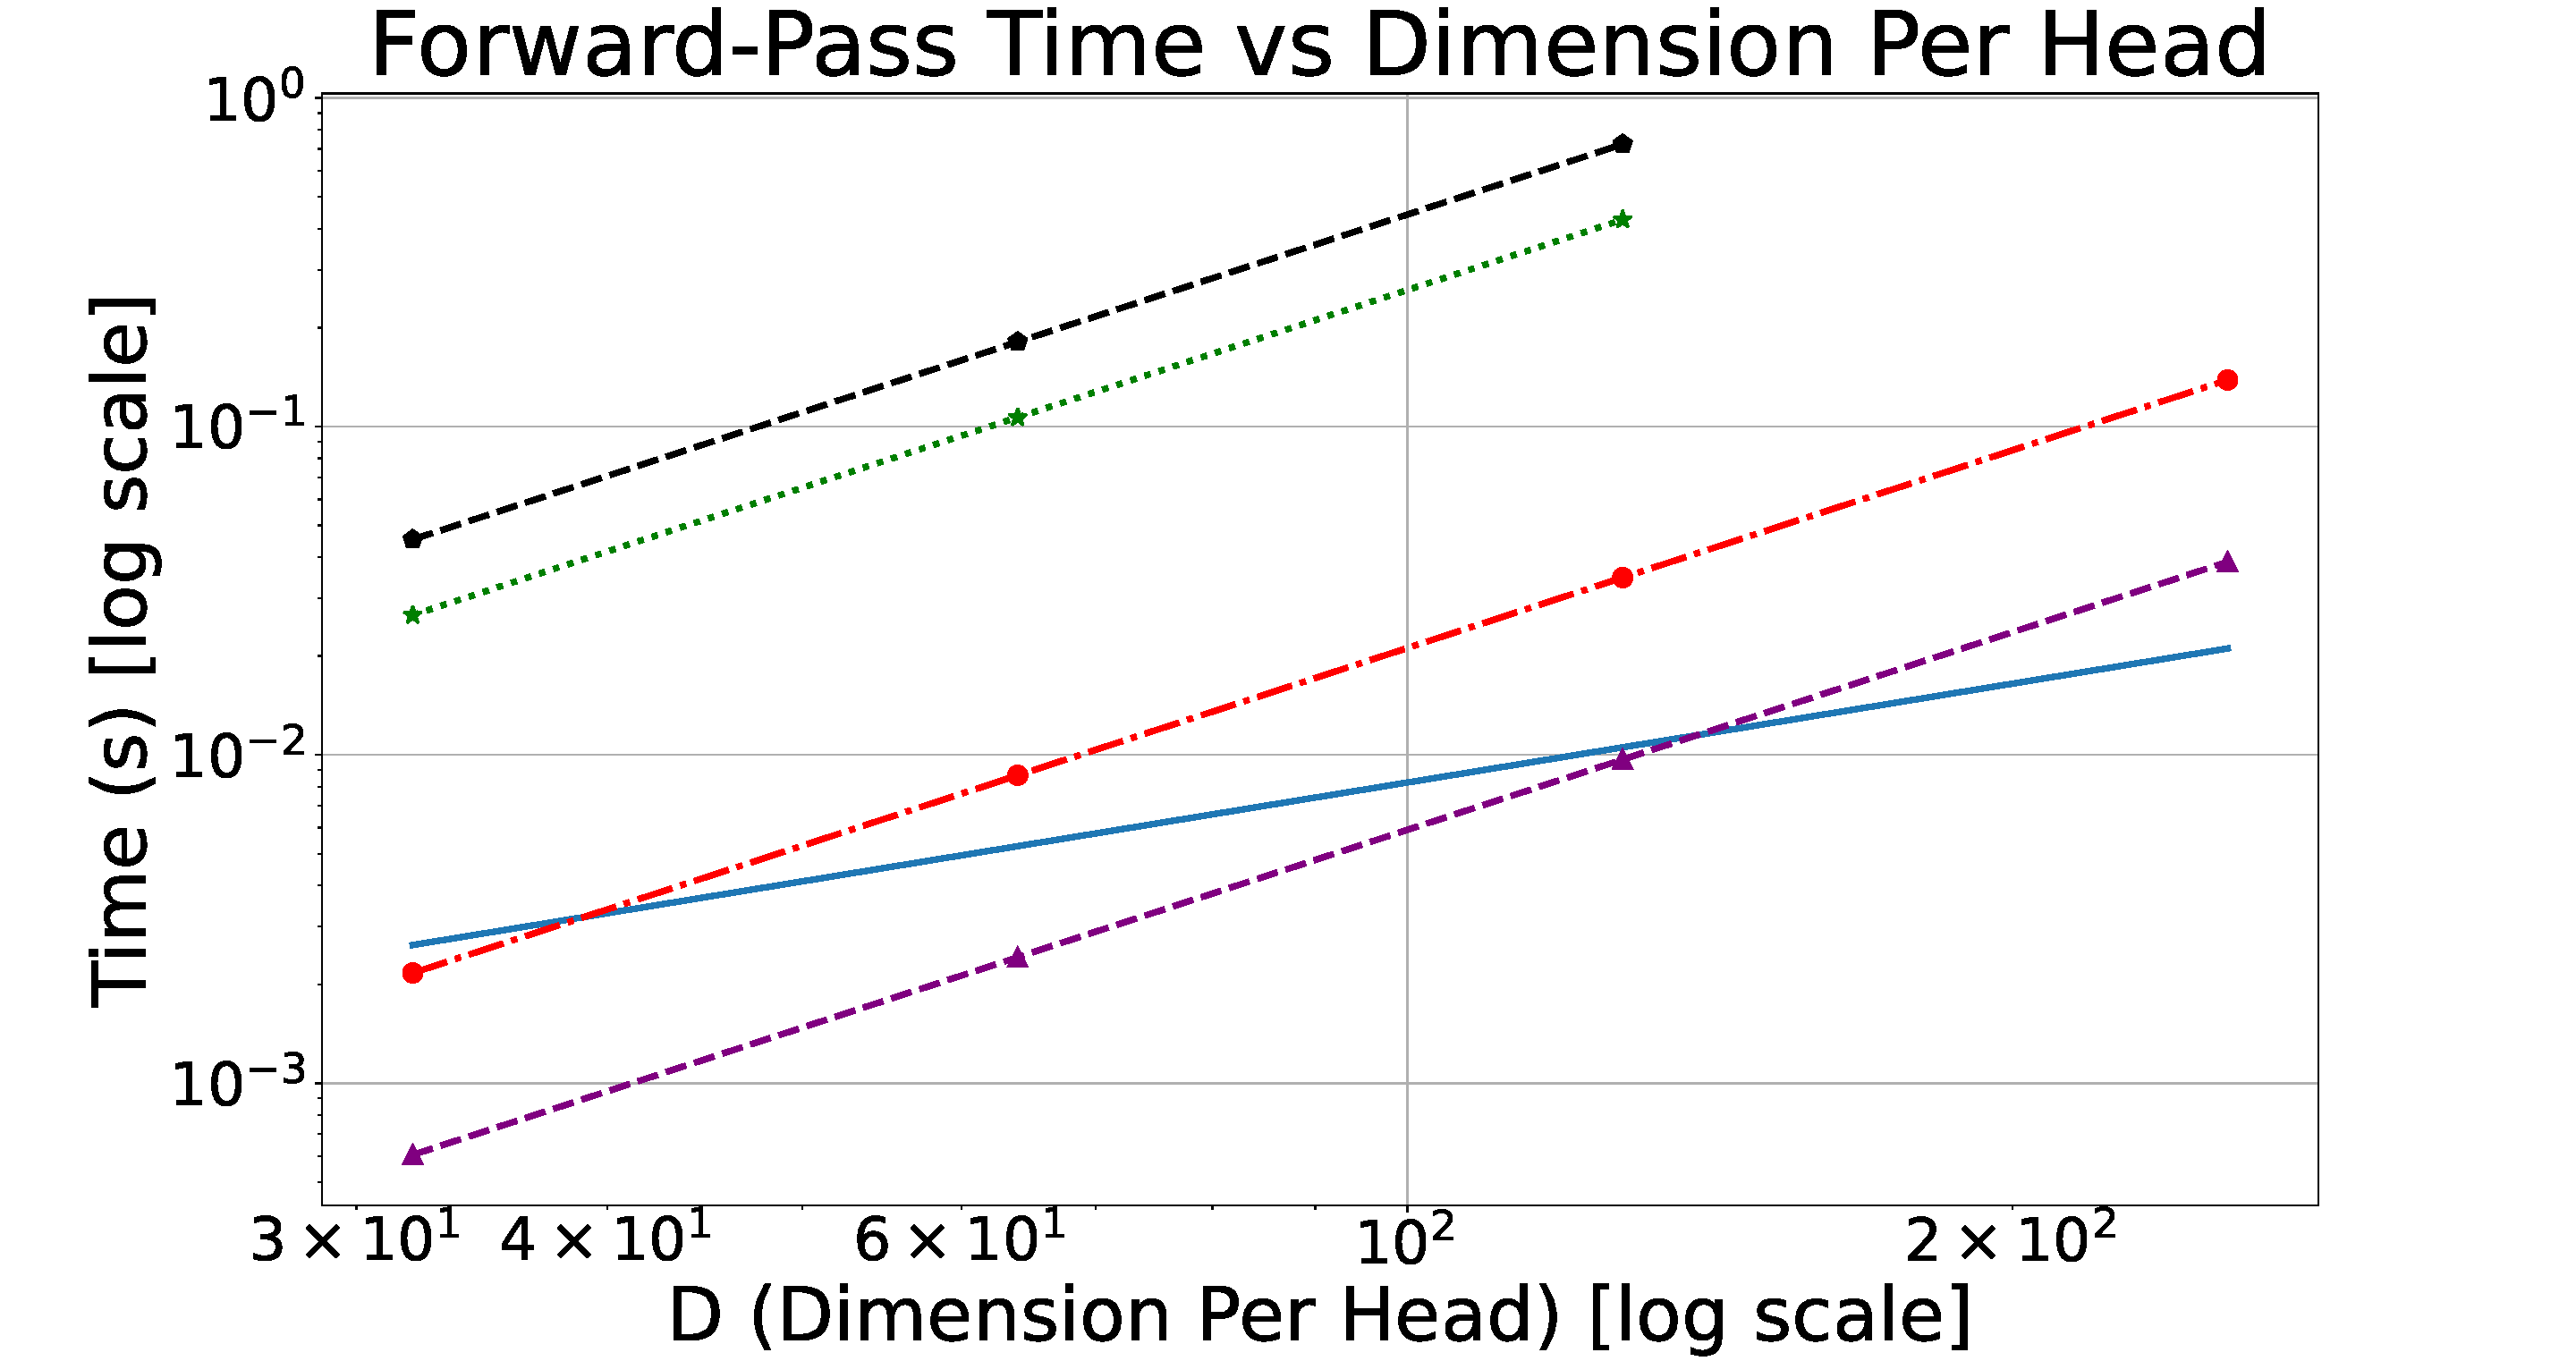
\includegraphics[width=\linewidth, trim=0mm 0mm 35mm 17mm, clip=true]{images/fp_tvd.pdf}
  \end{centering} \endminipage
\minipage{0.499\linewidth} \begin{centering}
\hspace{25pt}\textbf{FP Memory vs Dimension Per Head ($D$)}\par\medskip
  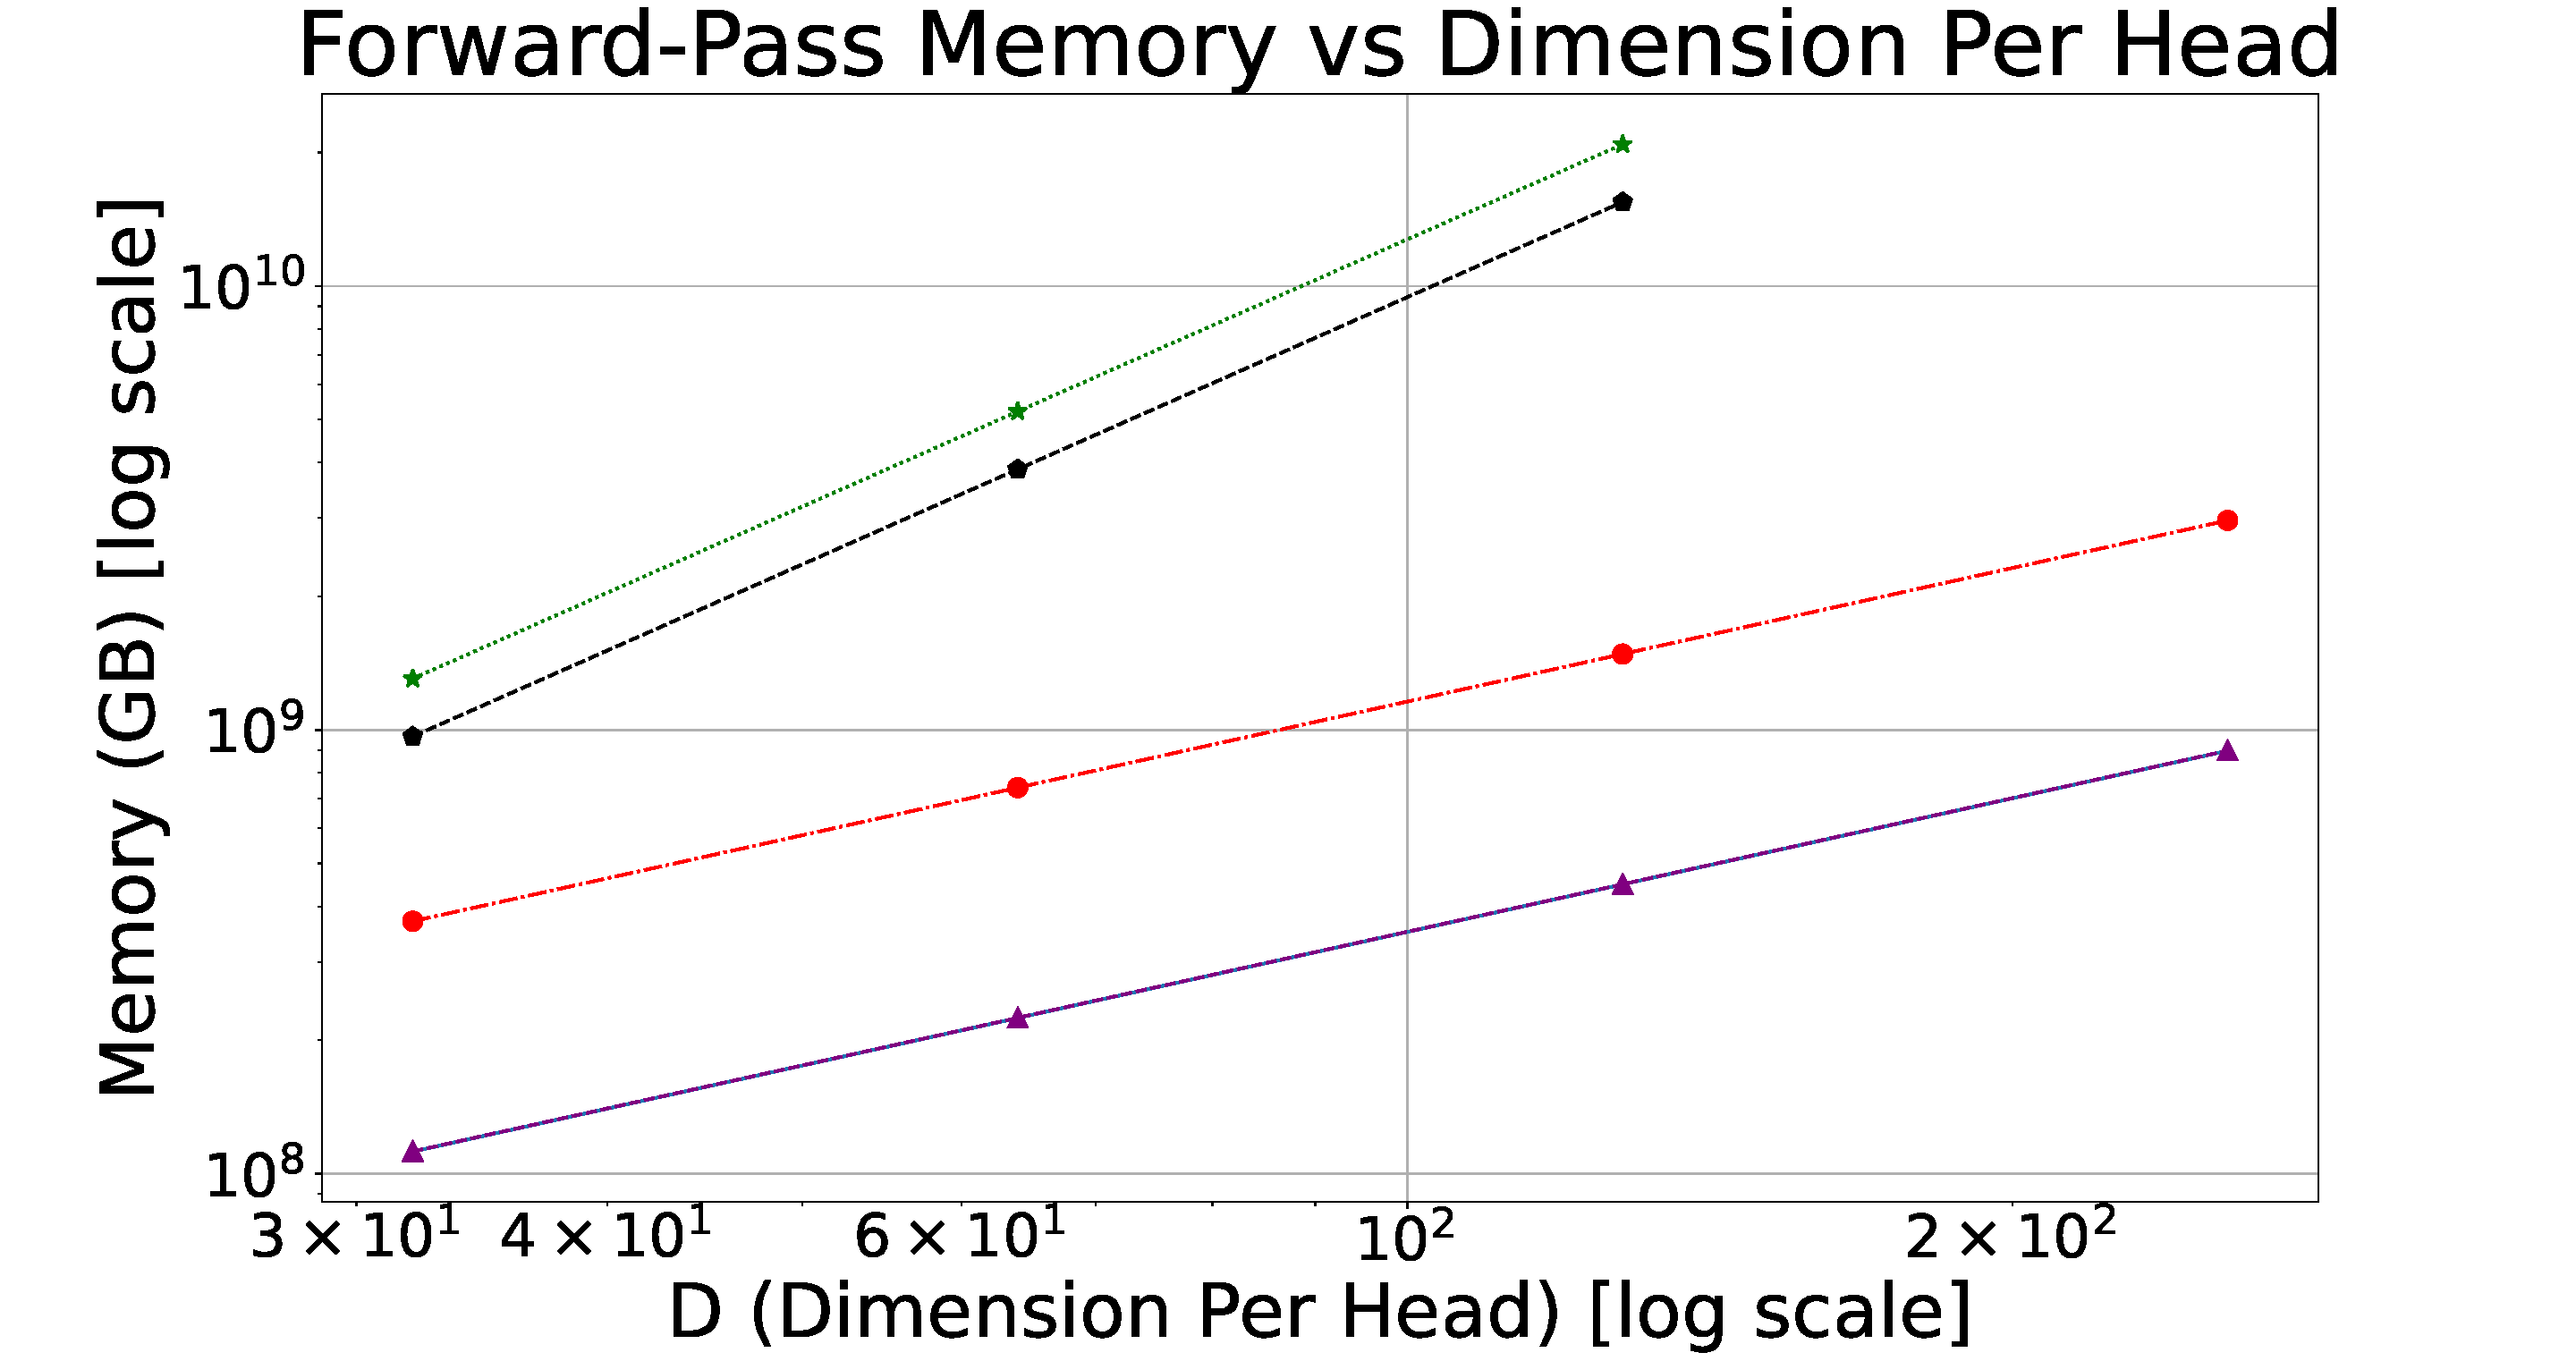
\includegraphics[width=\linewidth, trim=0mm 0mm 35mm 17mmmm, clip=true]{images/fp_mvd.pdf}
  \end{centering} \endminipage
\vspace{-10pt}
\caption{Time and memory scaling of our LA implementation, FlashAttention-2~\cite{dao2024flashattention} (Regular Attention), Gated LA~\cite{yang2023gated}, Speculative Decoding LA~\cite{you2024linear}, and baseline Pytorch LA implementation on an A6000 GPU during forward-pass (FP). The top two figures show the time and memory scaling as a function of number of tokens $N$ for dimension per head of $D = 128$, batch size $B=4$, and number of heads $H = 16$. The bottom two the figures show the scaling as a function of $D$ for $N = 4096$. The `Reg. Att.` and `Our LA` lines overlap in the memory scaling plots.}
\label{figforward}
\end{figure*}



\subsection{Standalone Layer}
\label{exp:forward}
The upper plots in Figure~\ref{figforward} show a log-log analysis of the time and memory complexity of a single attention head's forward-pass as a function of sequence length $N$, ranging from $10^3$ to $3×10^5$ tokens. These evaluations were conducted with a batch size of $B=4$, number of heads $H=16$ attention heads, and a per-head dimension of $D=128$, with the reported results representing the average of 100 iterations performed on an NVIDIA A6000 GPU and precision of float-32. The slopes observed in the plots indicate the order of dependency on $N$. All LA implementations exhibit a runtime scaling linearly with the number of tokens, while Regular Attention scales quadratically. Given the current trend of transformers scaling to $\sim 10^7$ context length, LA would be substantially more efficient. Furthermore, our implementation is $3.3\times$ faster than Gated LA. The observed performance improvement is attributed to our reduced data movement, and the implementation of LA using the Transformer architecture, in contrast to Gated LA's use of an RNN. Specifically, the inherent sequential structure of RNNs results in sequential computation of the output matrix, thereby limiting parallelization. In contrast, Transformers inherently allow for parallel computation of the output matrix. Moreover, the baseline and Spec. Dec. LA, which are based on Transformer architecture, are an order of magnitude slower, showcasing the effectiveness of our method and implementation. Regarding memory consumption, all implementations scale linearly with $N$. Our LA and Regular Attention have the lowest consumption, achieving $3.6\times$ less memory consumption than Gated LA and an order of magnitude lower than the baseline and Spec. Dec. LA.

\begin{figure*}[!h]
\minipage{0.499\linewidth} \begin{centering}
\hspace{25pt}\textbf{BP Time vs Sequence Length ($N$)}\par\medskip
  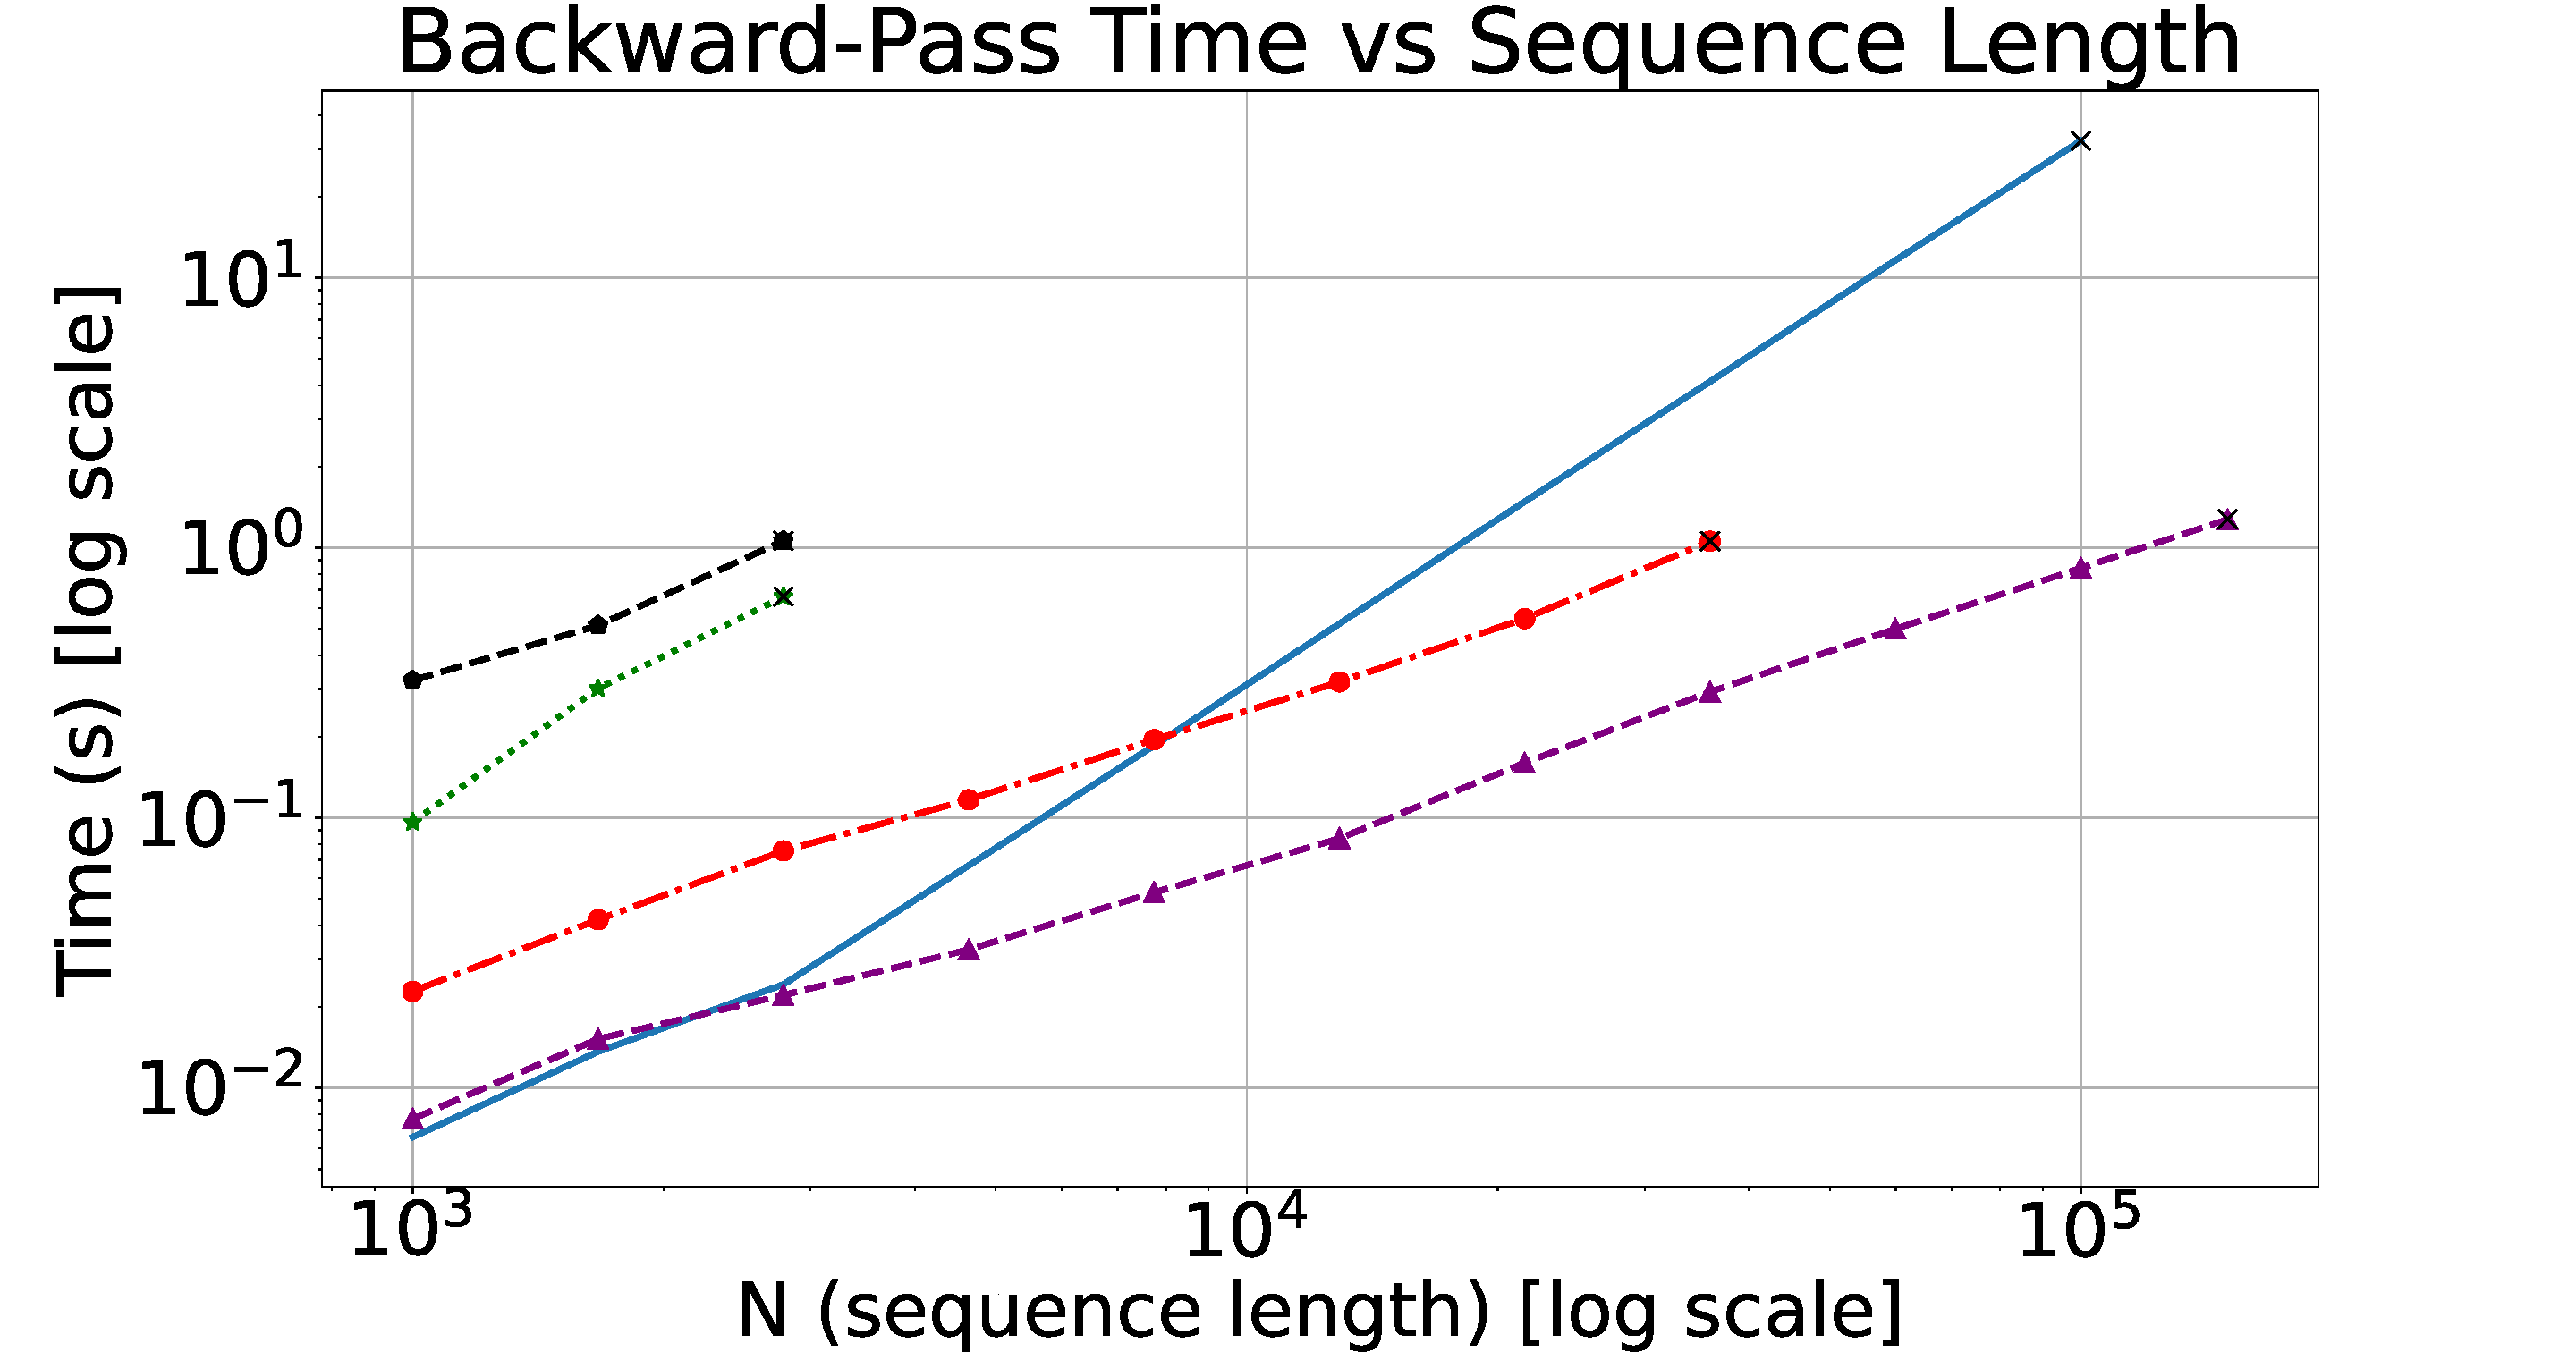
\includegraphics[width=\linewidth, trim=0mm 0mm 35mm 17mm, clip=true]{images/bp_tvn.pdf}
  \end{centering} \endminipage
\minipage{0.499\linewidth} \begin{centering}
\hspace{25pt}\textbf{BP Memory vs Sequence Length ($N$)}\par\medskip
  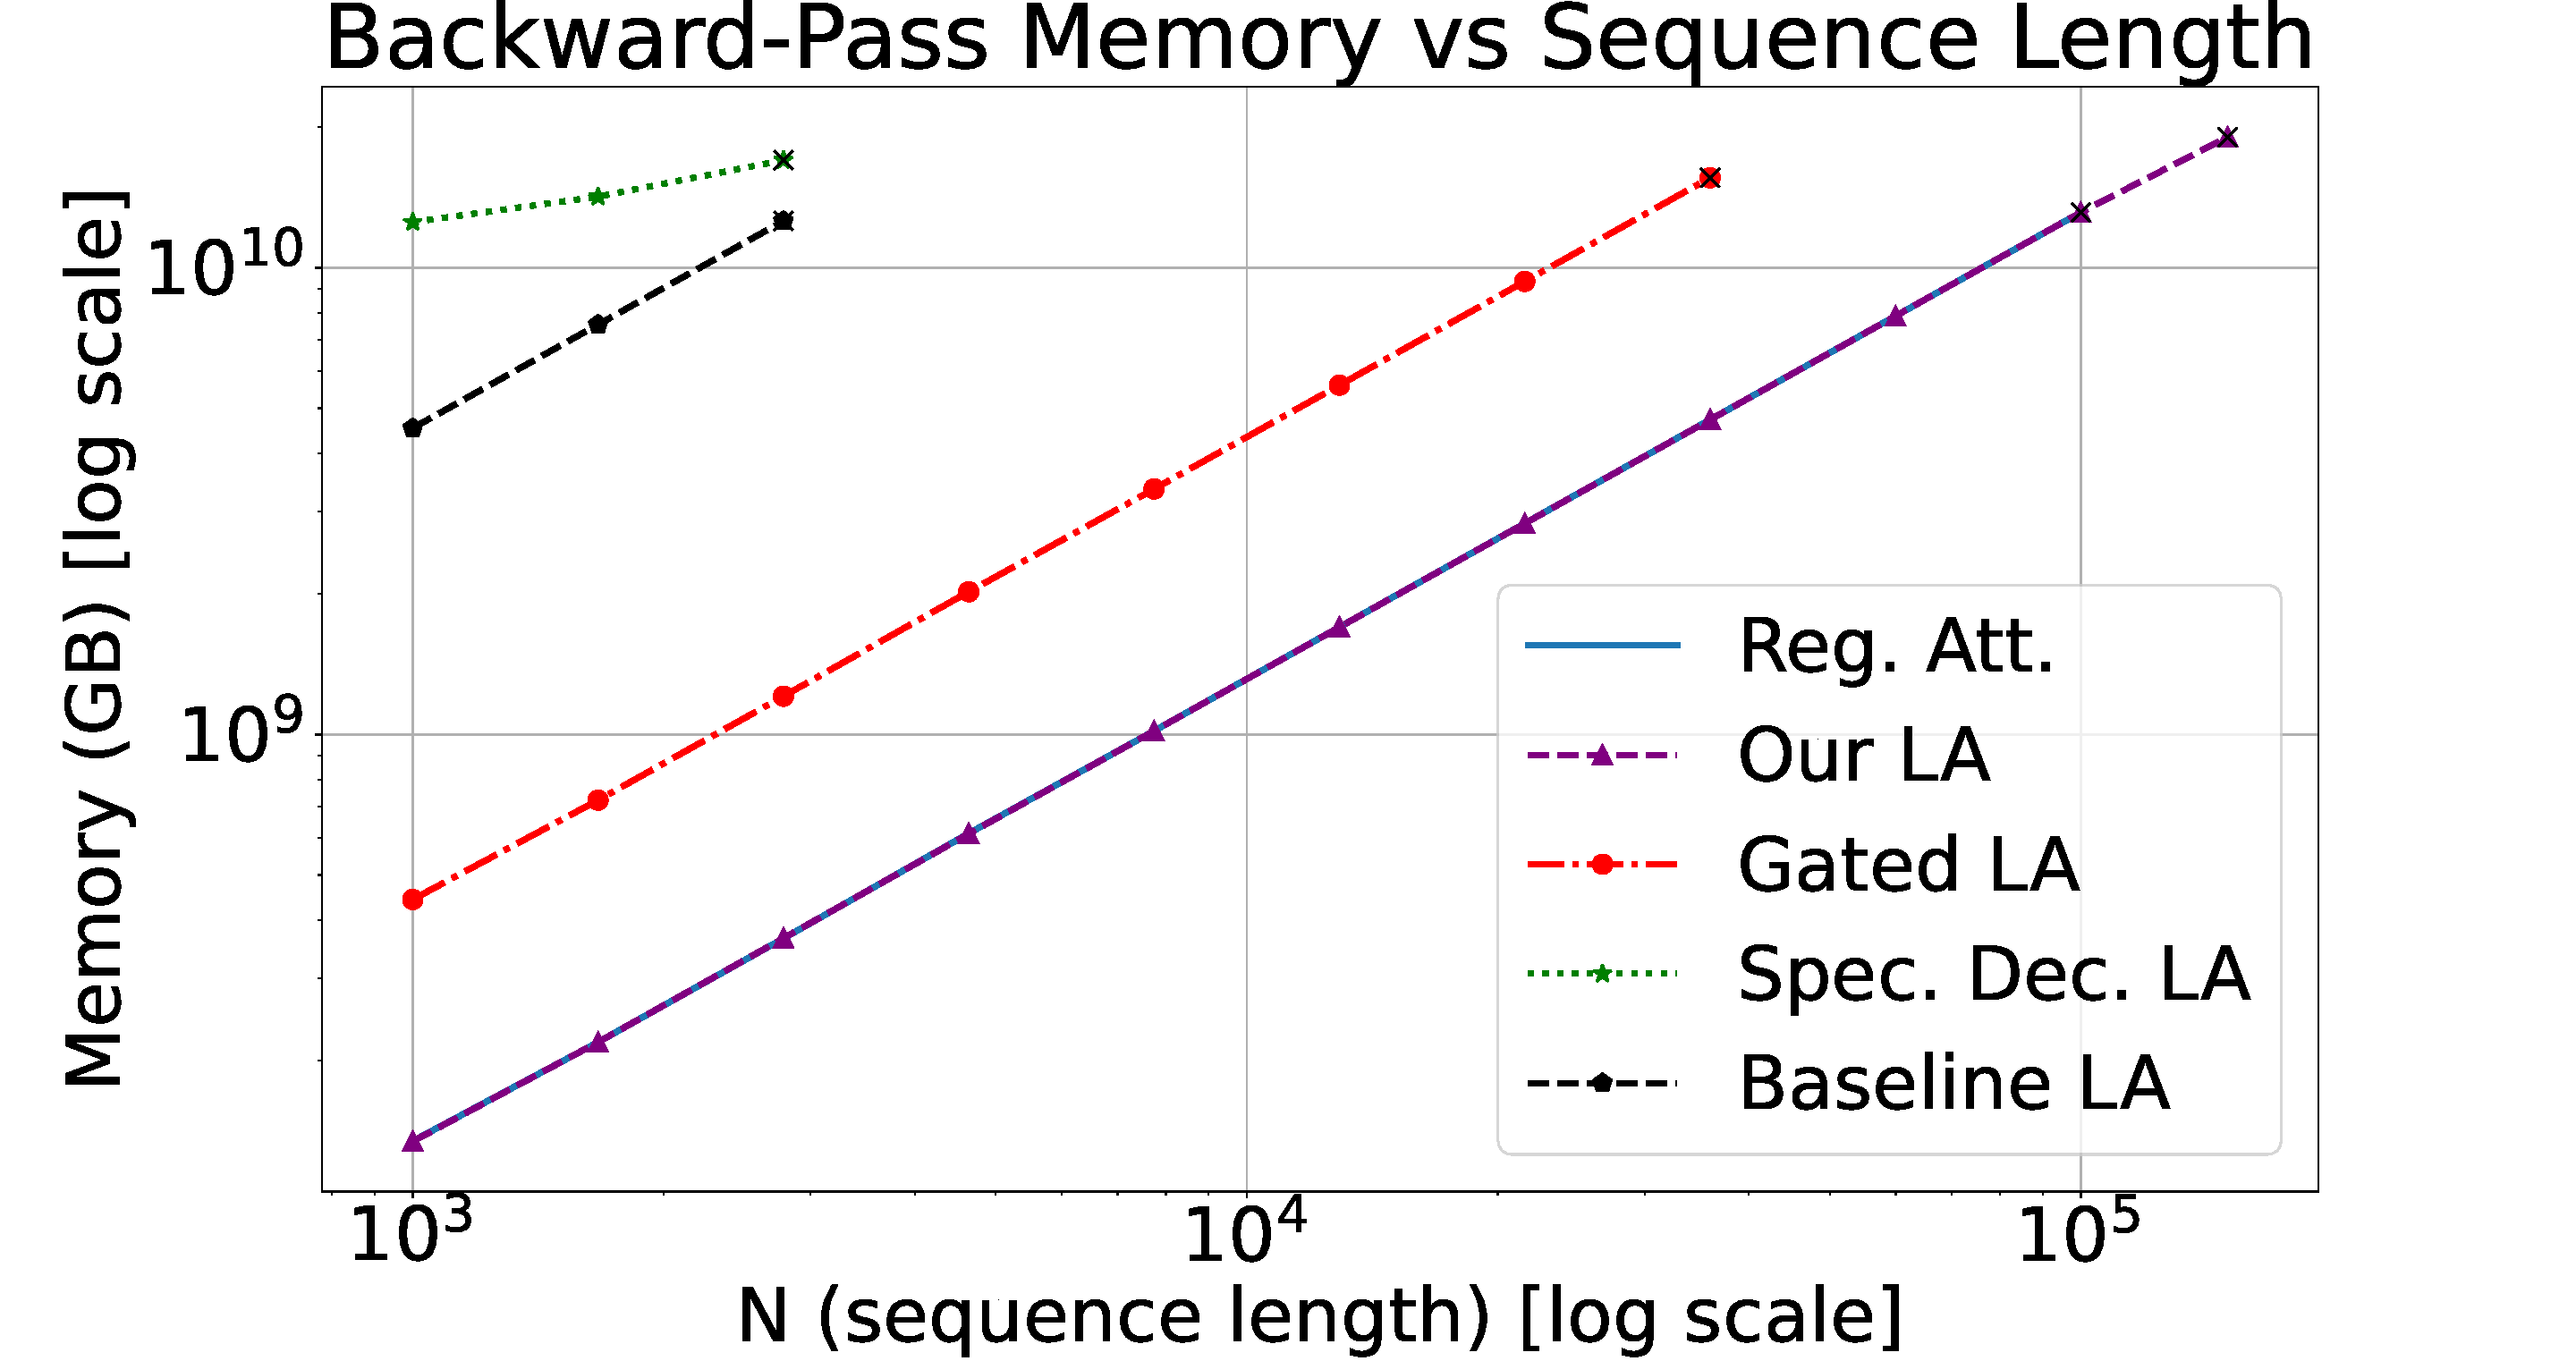
\includegraphics[width=\linewidth, trim=0mm 0mm 35mm 15mm, clip=true]{images/bp_mvn.pdf}
  \end{centering} \endminipage\hfill
% \vspace{20pt}
\minipage{0.499\linewidth} \begin{centering}
\hspace{25pt}\textbf{BP Time vs Dimension Per Head ($D$)}\par\medskip
  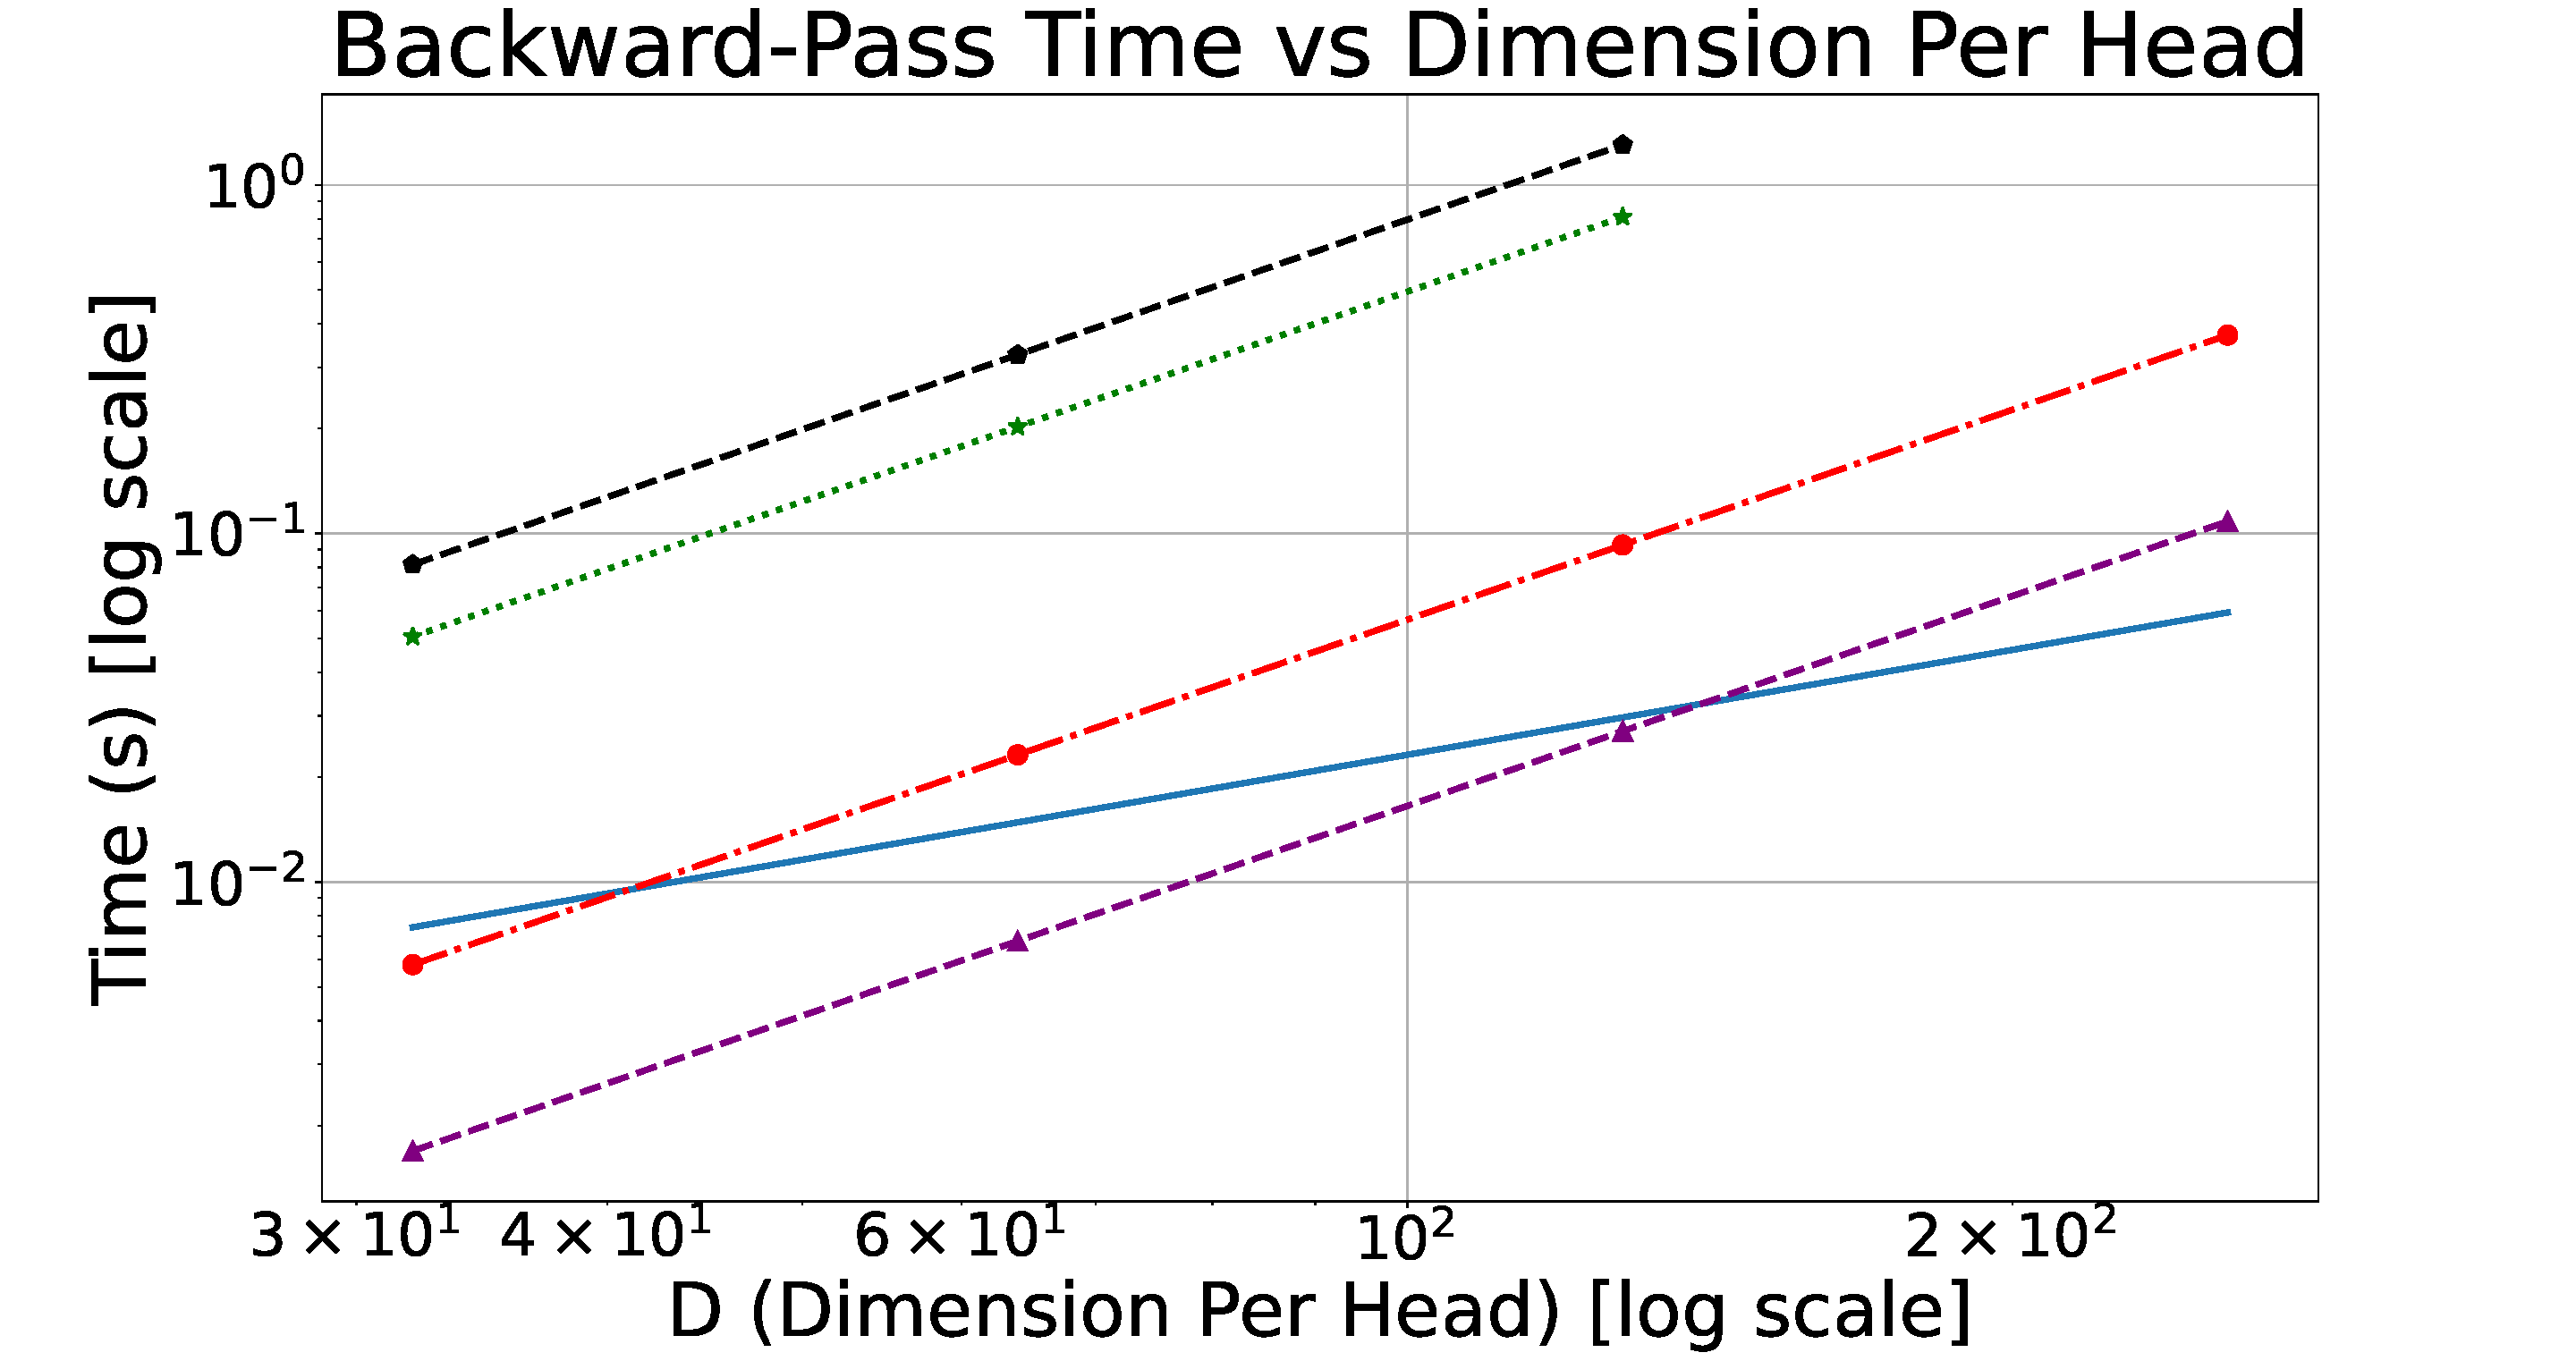
\includegraphics[width=\linewidth, trim=0mm 0mm 35mm 17mm, clip=true]{images/bp_tvd.pdf}
  \end{centering} \endminipage
\minipage{0.499\linewidth} \begin{centering}
\hspace{25pt}\textbf{BP Memory vs Dimension Per Head ($D$)}\par\medskip
  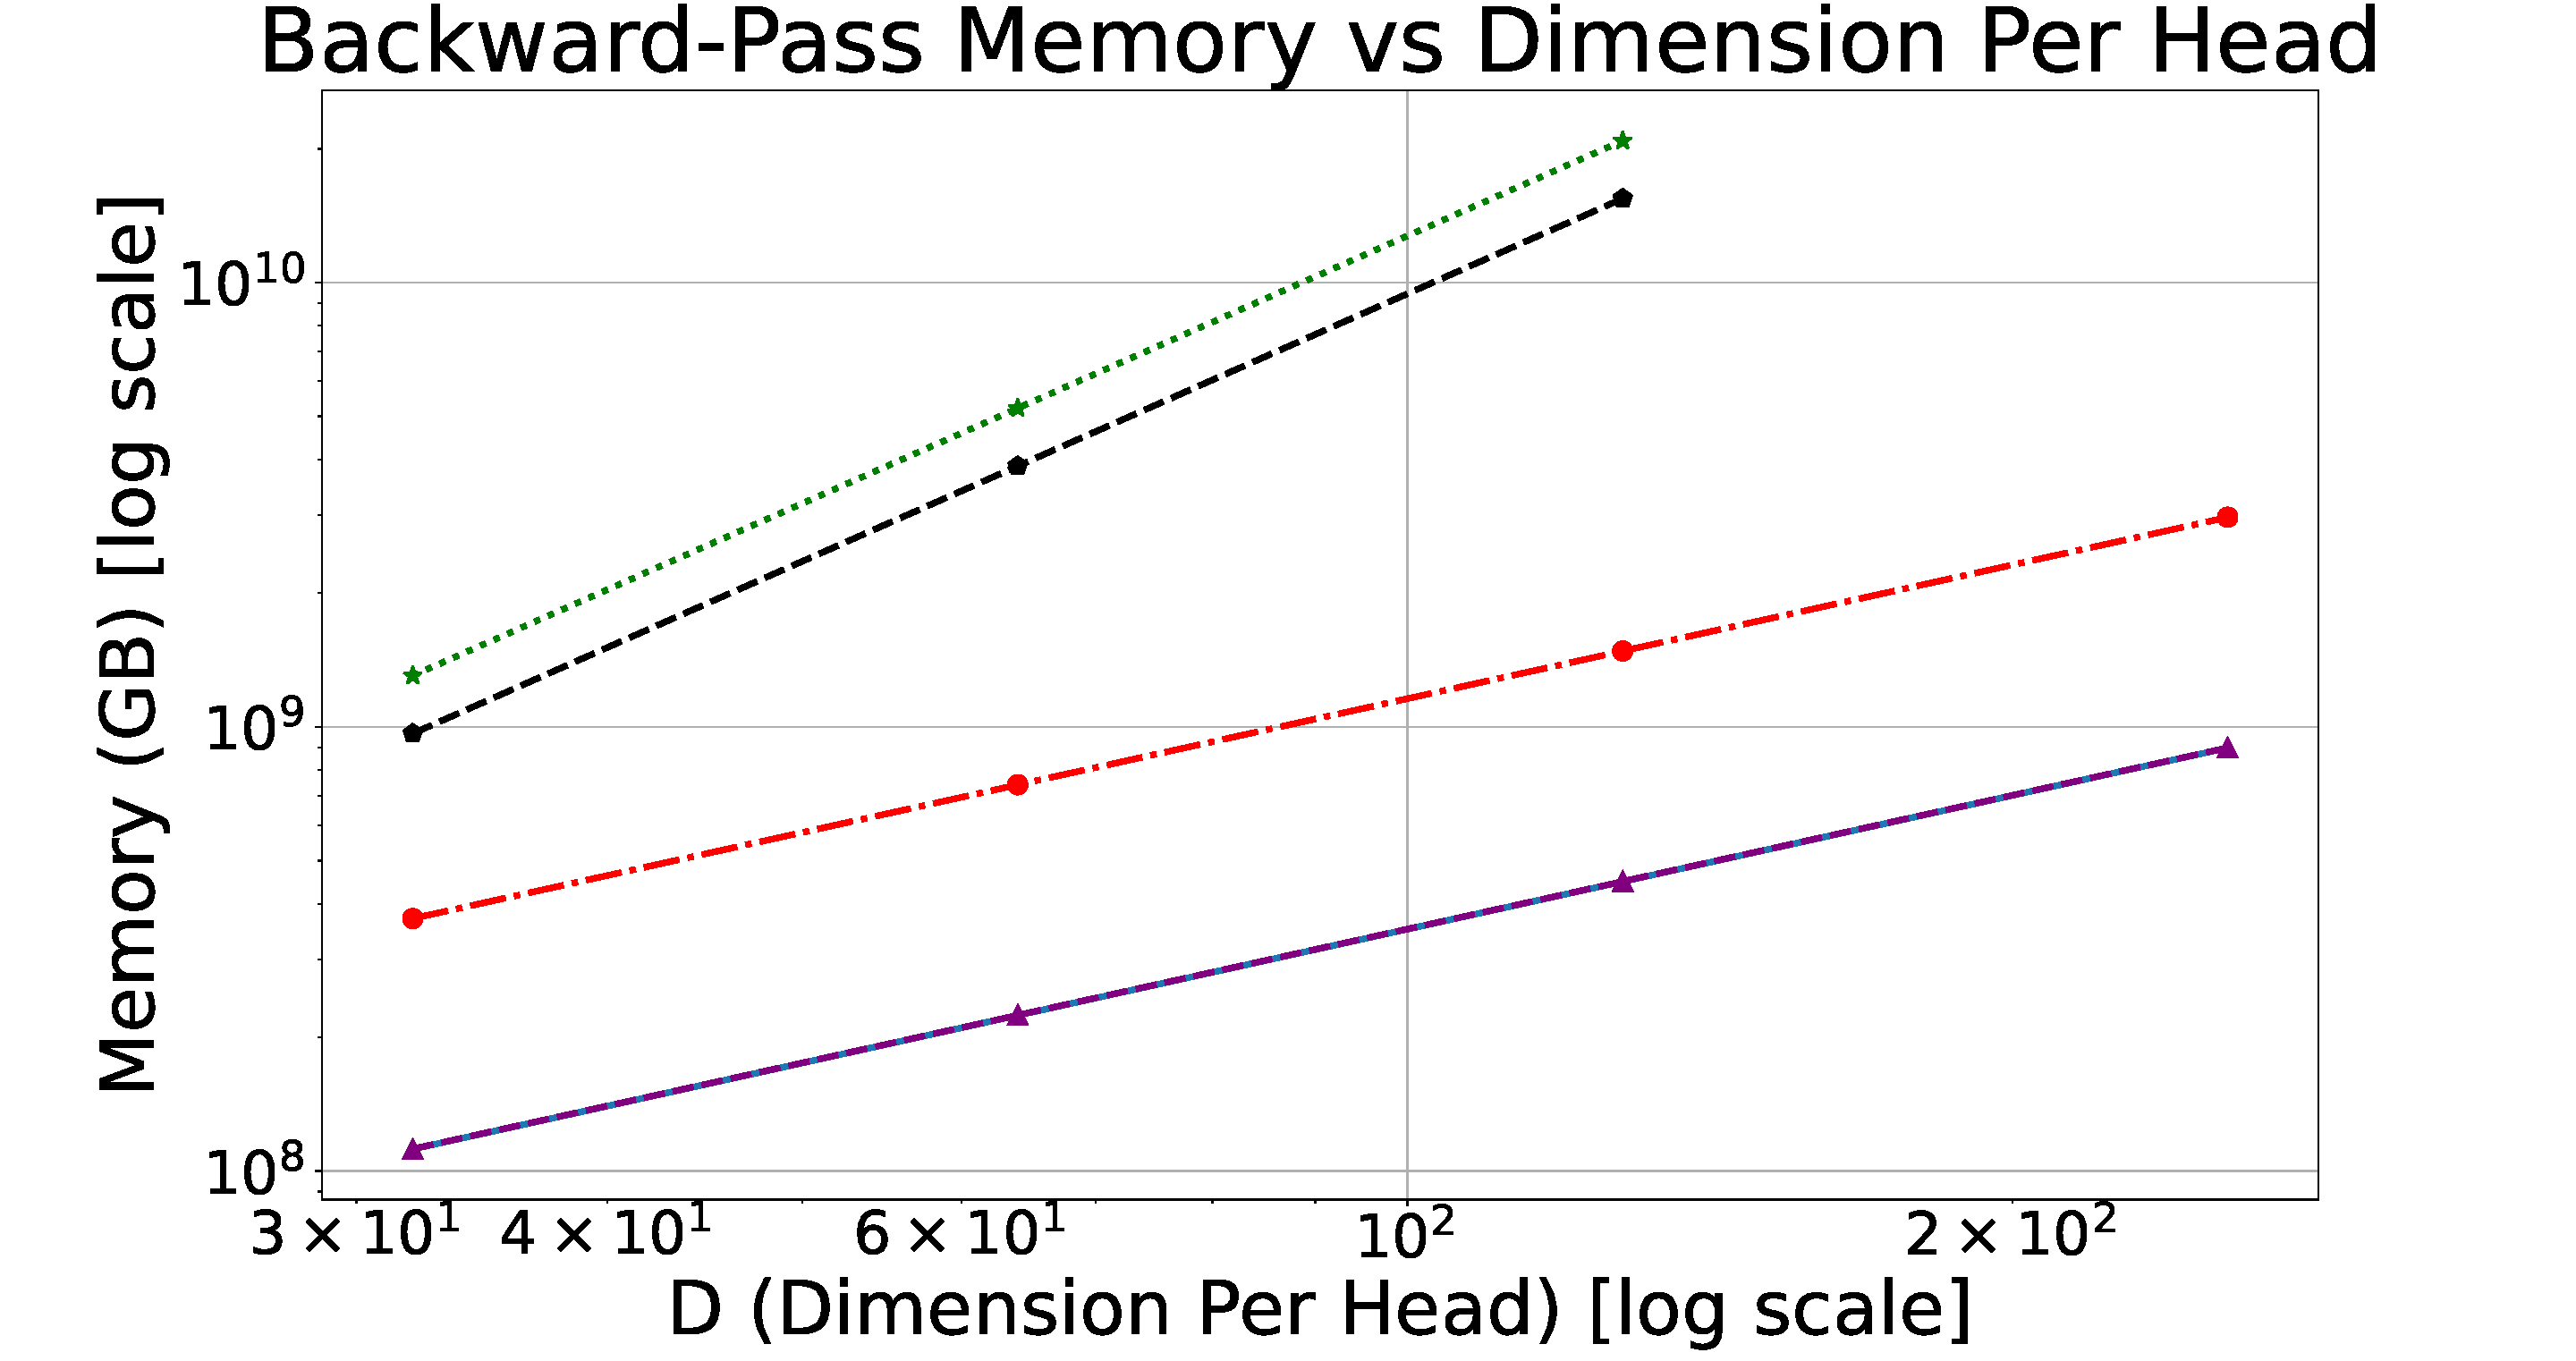
\includegraphics[width=\linewidth, trim=0mm 0mm 35mm 17mmmm, clip=true]{images/bp_mvd.pdf}
  \end{centering} \endminipage
\vspace{-10pt}
\caption{Time and memory scaling of our LA implementation, FlashAttention-2~\cite{dao2024flashattention} (Regular Attention), Gated LA~\cite{yang2023gated}, Speculative Decoding LA~\cite{you2024linear}, and baseline Pytorch LA implementation on an A6000 GPU during backward-pass (BP). The upper two figures show the time and memory scaling as a function of number of tokens $N$ for dimension per head of $D = 128$, batch size $B=4$, and number of heads $H = 16$. The bottom two the figures show the scaling as a function of $D$ for $N = 4096$. The `Reg. Att.` and `Our LA` lines overlap in the memory scaling plots.}
\label{figbackward}
\end{figure*}

\par The bottom plots in Figure~\ref{figforward} show the time and memory scaling of an attention head against dimension per head $D$ under the same setting, except $32\leq D\leq 256$ and $N = 4096$. All of the LA implementations have a runtime scaling quadratcially with dimension per head, whereas Regular Attention scales linearly. Fortunately, the dimension per head is a constant parameter ($~10^2$) in the Transformer architecture, and is relatively small ($D<<N$). As for the memory consumption, Our LA, Gated LA and Regular Attention have a linear scaling with $D$, whereas baseline and Spec. Dec. LA scale quadratically. This quadratic scaling arises from the application of a causal mask. To be specific, relying on a differentiable programming library to derive the backward-pass for LA with a causal mask results in $O(ND^2)$ memory complexity, as discussed in Section~\ref{custom_gradients}. In contrast, Our LA and Gated LA employ manually derived backward-passes. 

\par The upper and bottom plots in Figure~\ref{figbackward} show the time and memory scaling for a single backward-pass under the same setting as above against $N$ and $D$ respectively. The scaling trends mirror those observed in the forward-pass. Specifically, Regular Attention exhibits a quadratic runtime scaling, while the LA implementations demonstrate linear scaling, with our implementation significantly outperforming other LA variants in terms of time and memory consumption. 

\par Figure~\ref{figdatatime} presents the ratio of time spent on data movement (primarily off-chip memory read/write) to the total runtime (left), and the total data movement time (right) for LA implementations averaged over 100 runs on an A6000. Our method allows for a computational pattern that maximizes data reuse rate, and our implementation achieves this efficiency through specific thread scheduling and data movement, as elaborated in Section~\ref{sec4}. As a result, our implementation exhibits minimal data movement. Compared to other LA implementations, the portion of time spent on data movement is significantly lower, where it is roughly one-third of the next lowest ratio, observed in Gated LA $(71\%)$. This optimized data movement becomes even more apparent when examining the total data movement time, where our implementation achieves an order of magnitude reduction compared to the next best, Gated LA.

\begin{figure}[!h]
  \centering
  \hspace{0pt}\textbf{Data Movement to Total Time Ratio}\hspace{60pt}\textbf{Time Spent on Data Movement}\par\medskip
  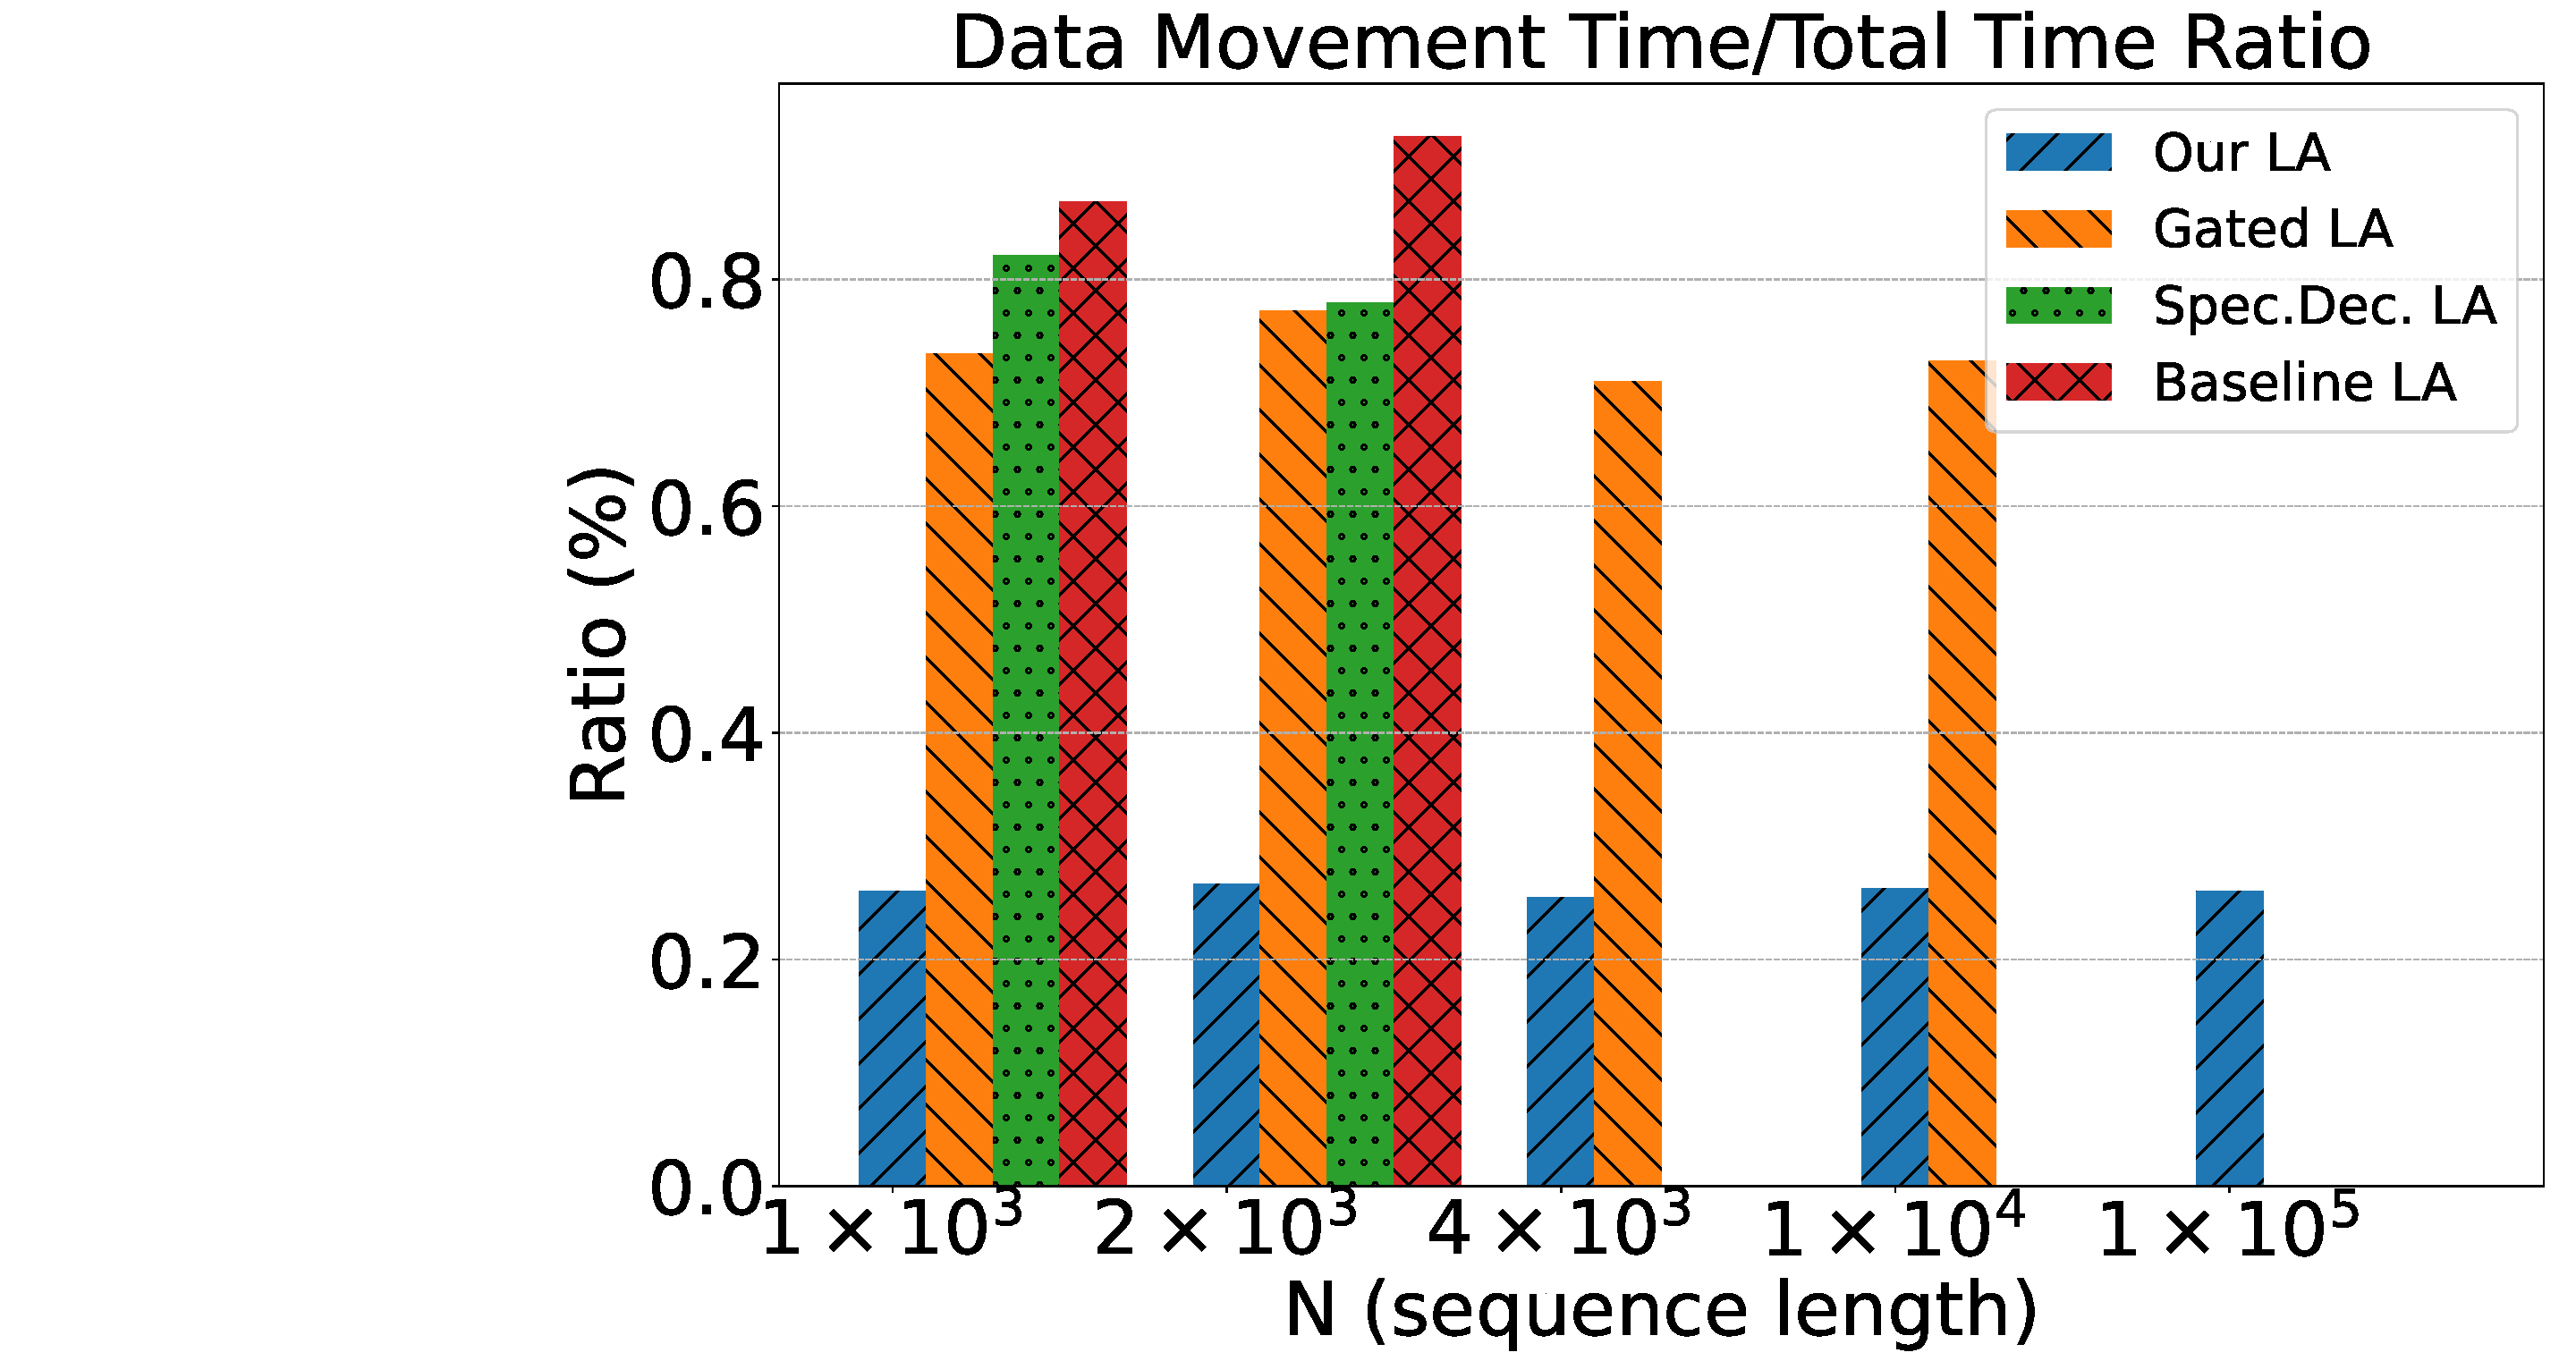
\includegraphics[width=0.49\linewidth, trim=95mm 0mm 0mm 15mm, clip=true]{images/ratio_time.pdf}
  % \hspace{35pt}\textbf{Time Spent in Data Movement - Forward-Pass}\par\medskip
  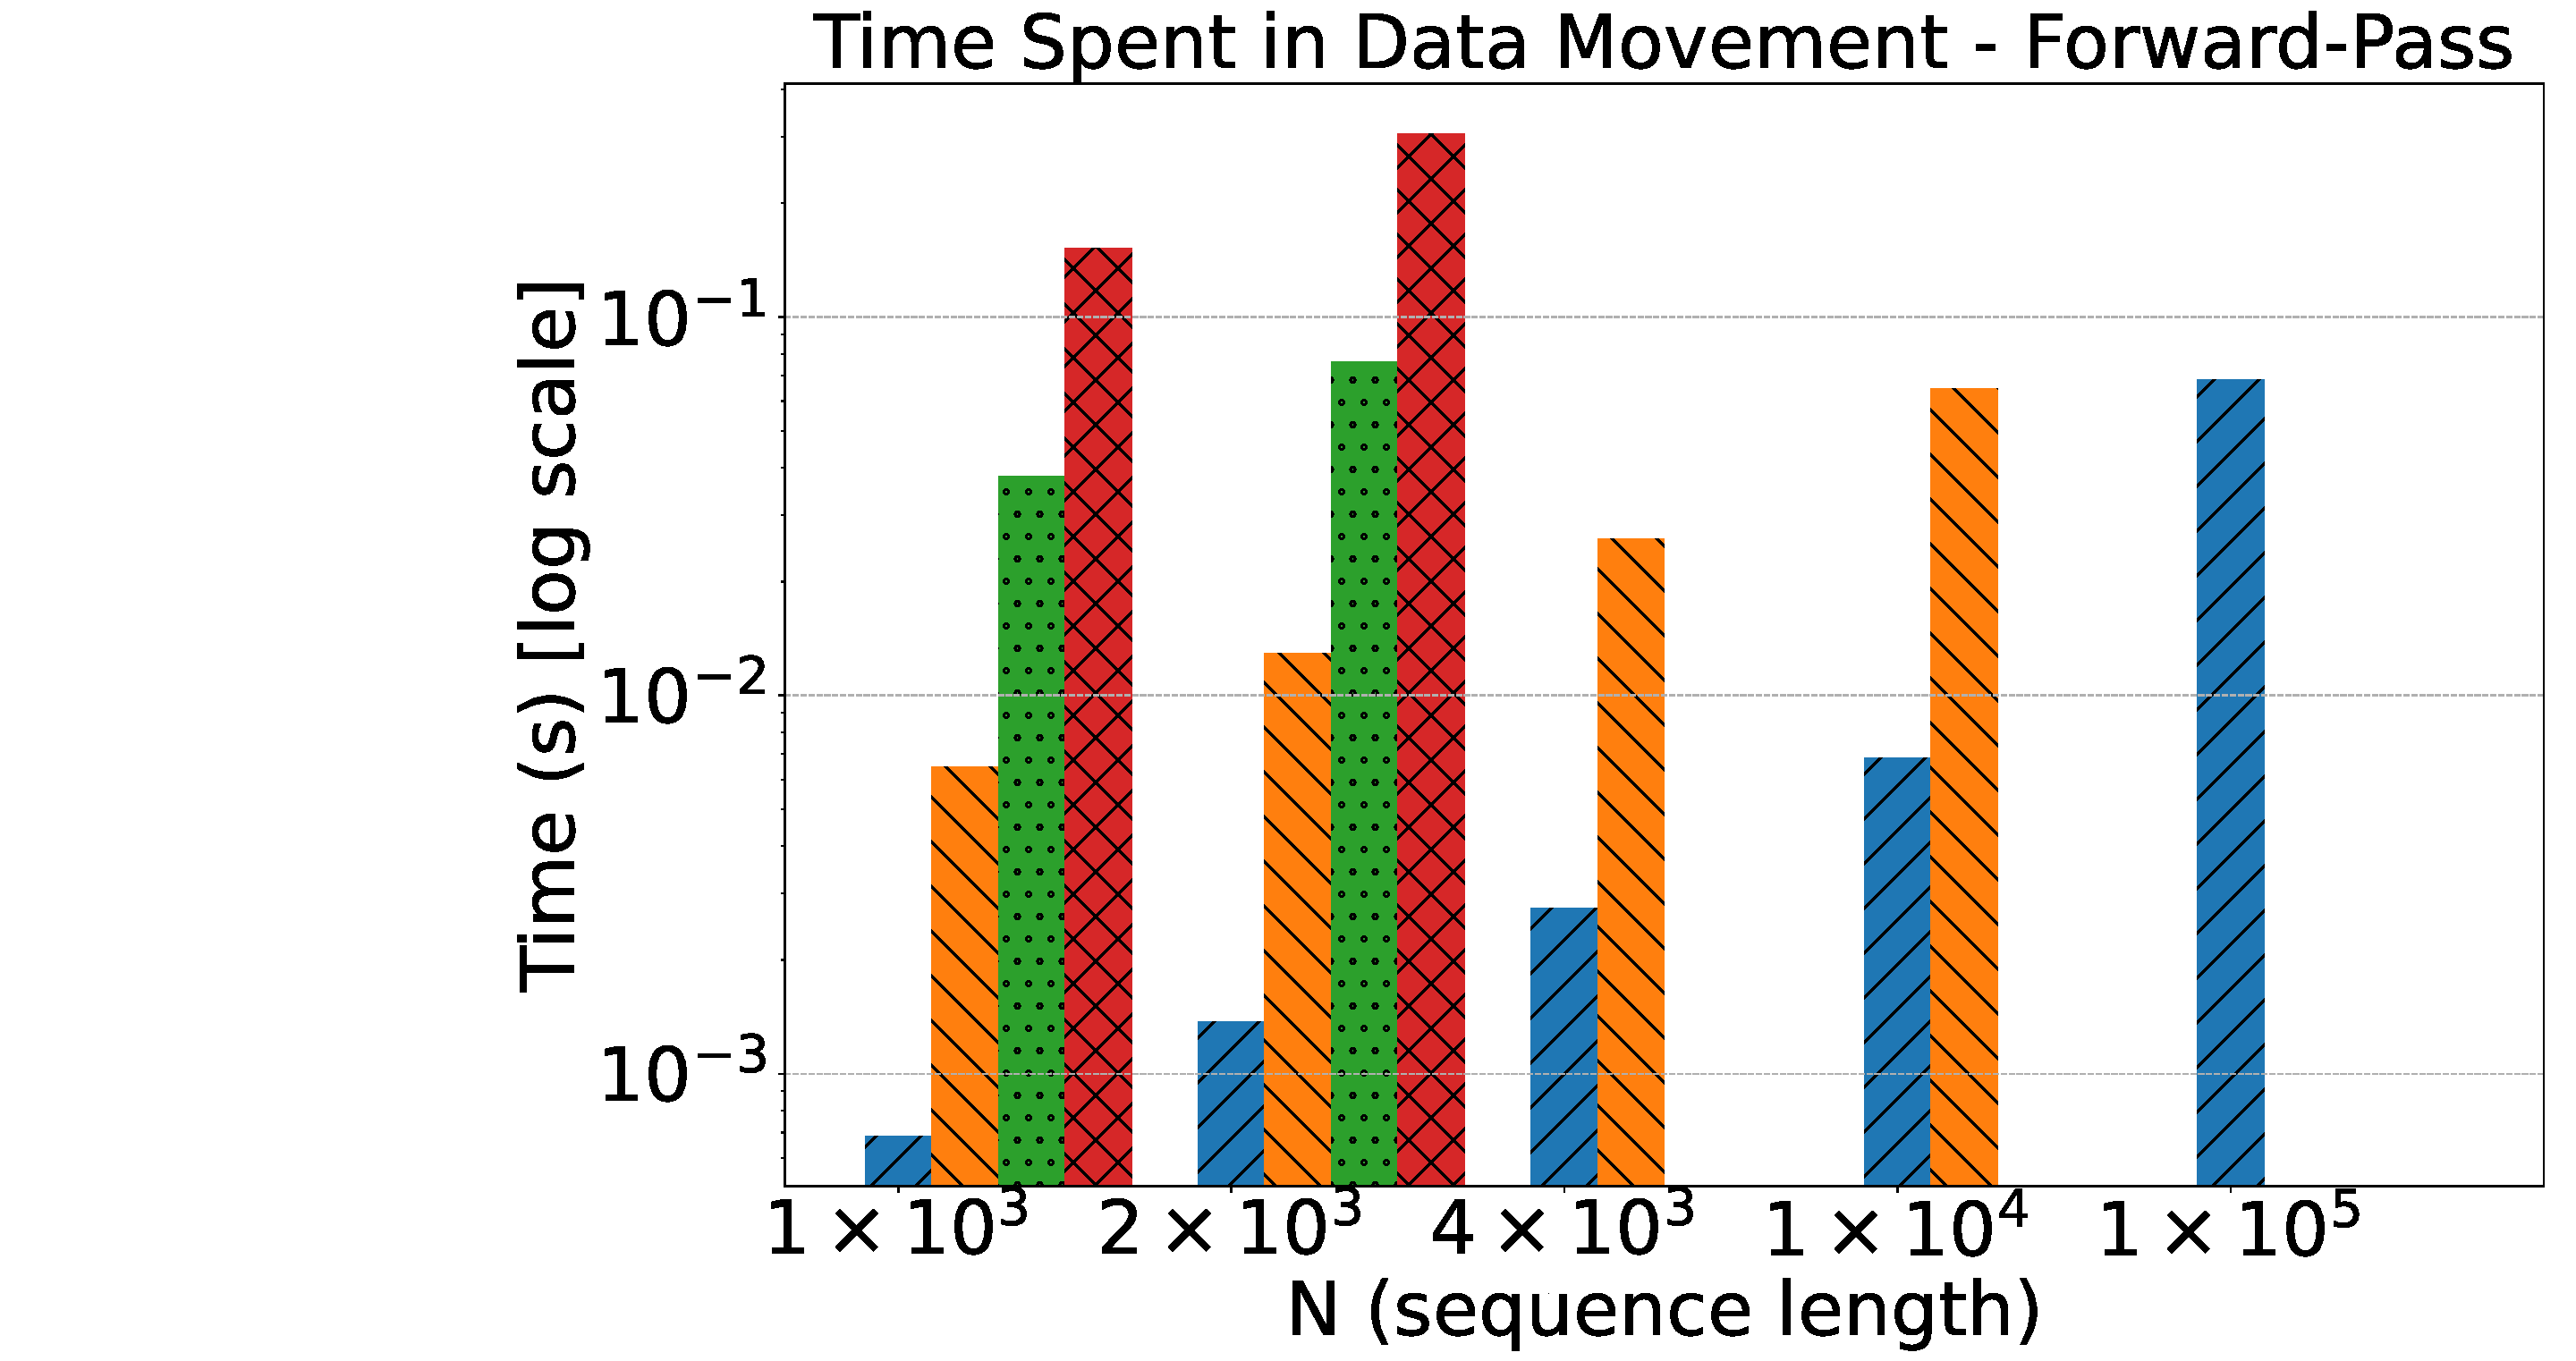
\includegraphics[width=0.49\linewidth, trim=95mm 0mm 0mm 15mm, clip=true]{images/data_time.pdf}
  % \hspace{30pt}\textbf{Time Spent in Data Movement - Backward-Pass}\par\medskip
  % \includegraphics[width=0.33\linewidth, trim=95mm 0mm 0mm 16mm, clip=true]{images/databp_time.pdf}
  \caption{Ratio of data movement time to total runtime (left), and total data movement time for the forward-pass (right) across various sequence lengths for LA implementations. Empty bars indicate out of memory. Our approach minimizes data movement, resulting in significantly lower ratio and movement time.}
  \label{figdatatime} 
\end{figure}

\par Compared to baseline LA implementation, where default Pytorch functions are used, the difference is a staggering $100\times$. This significant gap arises from the inherent limitations of differentiable programming libraries. More precisely, to derive gradients during the backward-pass, these libraries must store every operation within a computational graph and apply the `Chain Rule`. This approach becomes highly inefficient for element-wise operations, especially with extremely large data dimensions, as storing operations for each element results in a massive graph. Instead, tensor-wise operations should be employed, where the same operation is applied to the entire tensor and can be stored efficiently in the graph. However, the drawback of tensor-wise operations is that they restrict the flexibility of calculation patterns, and each such operation necessitates a read/write access to off-chip memory, which is extremely slow and can take hundreds of cycles. On the A6000 architecture, off-chip memory access typically ranges from 300 to 800 cycles, depending on memory traffic. In contrast, a custom CUDA implementation grants us the freedom to implement intricate computational and data movement patterns, which in turn enables optimized implementations, such as the one described in Section~\ref{sec4}.


\par In conclusion, our implementation scales linearly with $N$ and $D$ in terms of both time and memory, achieving a $3.3\times$ faster runtime and $3.6\times$ lower memory consumption compared to Gated LA, the state-of-the-art LA implementation. In comparison to efficient I/O-aware Regular Attention implementation FlashAttention-2, our approach demonstrates a faster runtime for $N>3000$ while maintaining similar memory consumption.




\subsection{Training an LLM}
\label{exp:llm}
To demonstrate the usefulness of our LA in practice, we train an LLM on the English partition of Wiki-40B~\cite{guo2020wiki}. We chose Pythia-1.4B~\cite{biderman2023pythia} as our LLM architecture with a token length of $N = 8192$. We deployed our model using LitGPT~\cite{litgpt-2023} using eight A6000 GPUs. We use rotary positional encoding~\cite{su2024roformer}, cosine warmup and decay with a minimum and maximum learning rate of $5e-5$ and $1e-3$, and global batch size of $256$. We train the model using our implementation of LA, Gated LA, and Regular Attention (FlashAttention-2). The hyperparameters used are the same for both methods. 
The plots in Figure~\ref{curve} show the learning curves for training loss as a function of wall-clock time (left) and training step (right). Compared to Regular Attention, both LA implementations have a slower convergence based on iteration count. However, they converge to the same loss, hinting to the fact that LA has comparable expresivity to Regular Attention. As for wall-clock time, our LA implementation exhibits substantial speedup of $2.8\times$ compared to Gated LA. Compared to Regular Attention, we exhibit $1.8\times$ speedup. The latter is attributed to $O(N)$ time scaling of LA, as opposed to Regular Attention's scaling of $O(N^2)$. 

\begin{figure}[!h]
  \centering
  
  \hspace{0pt}\textbf{Learning Curve - Wall-Clock Time}\hspace{72pt}\textbf{Learning Curve -Training Step}\par\medskip
  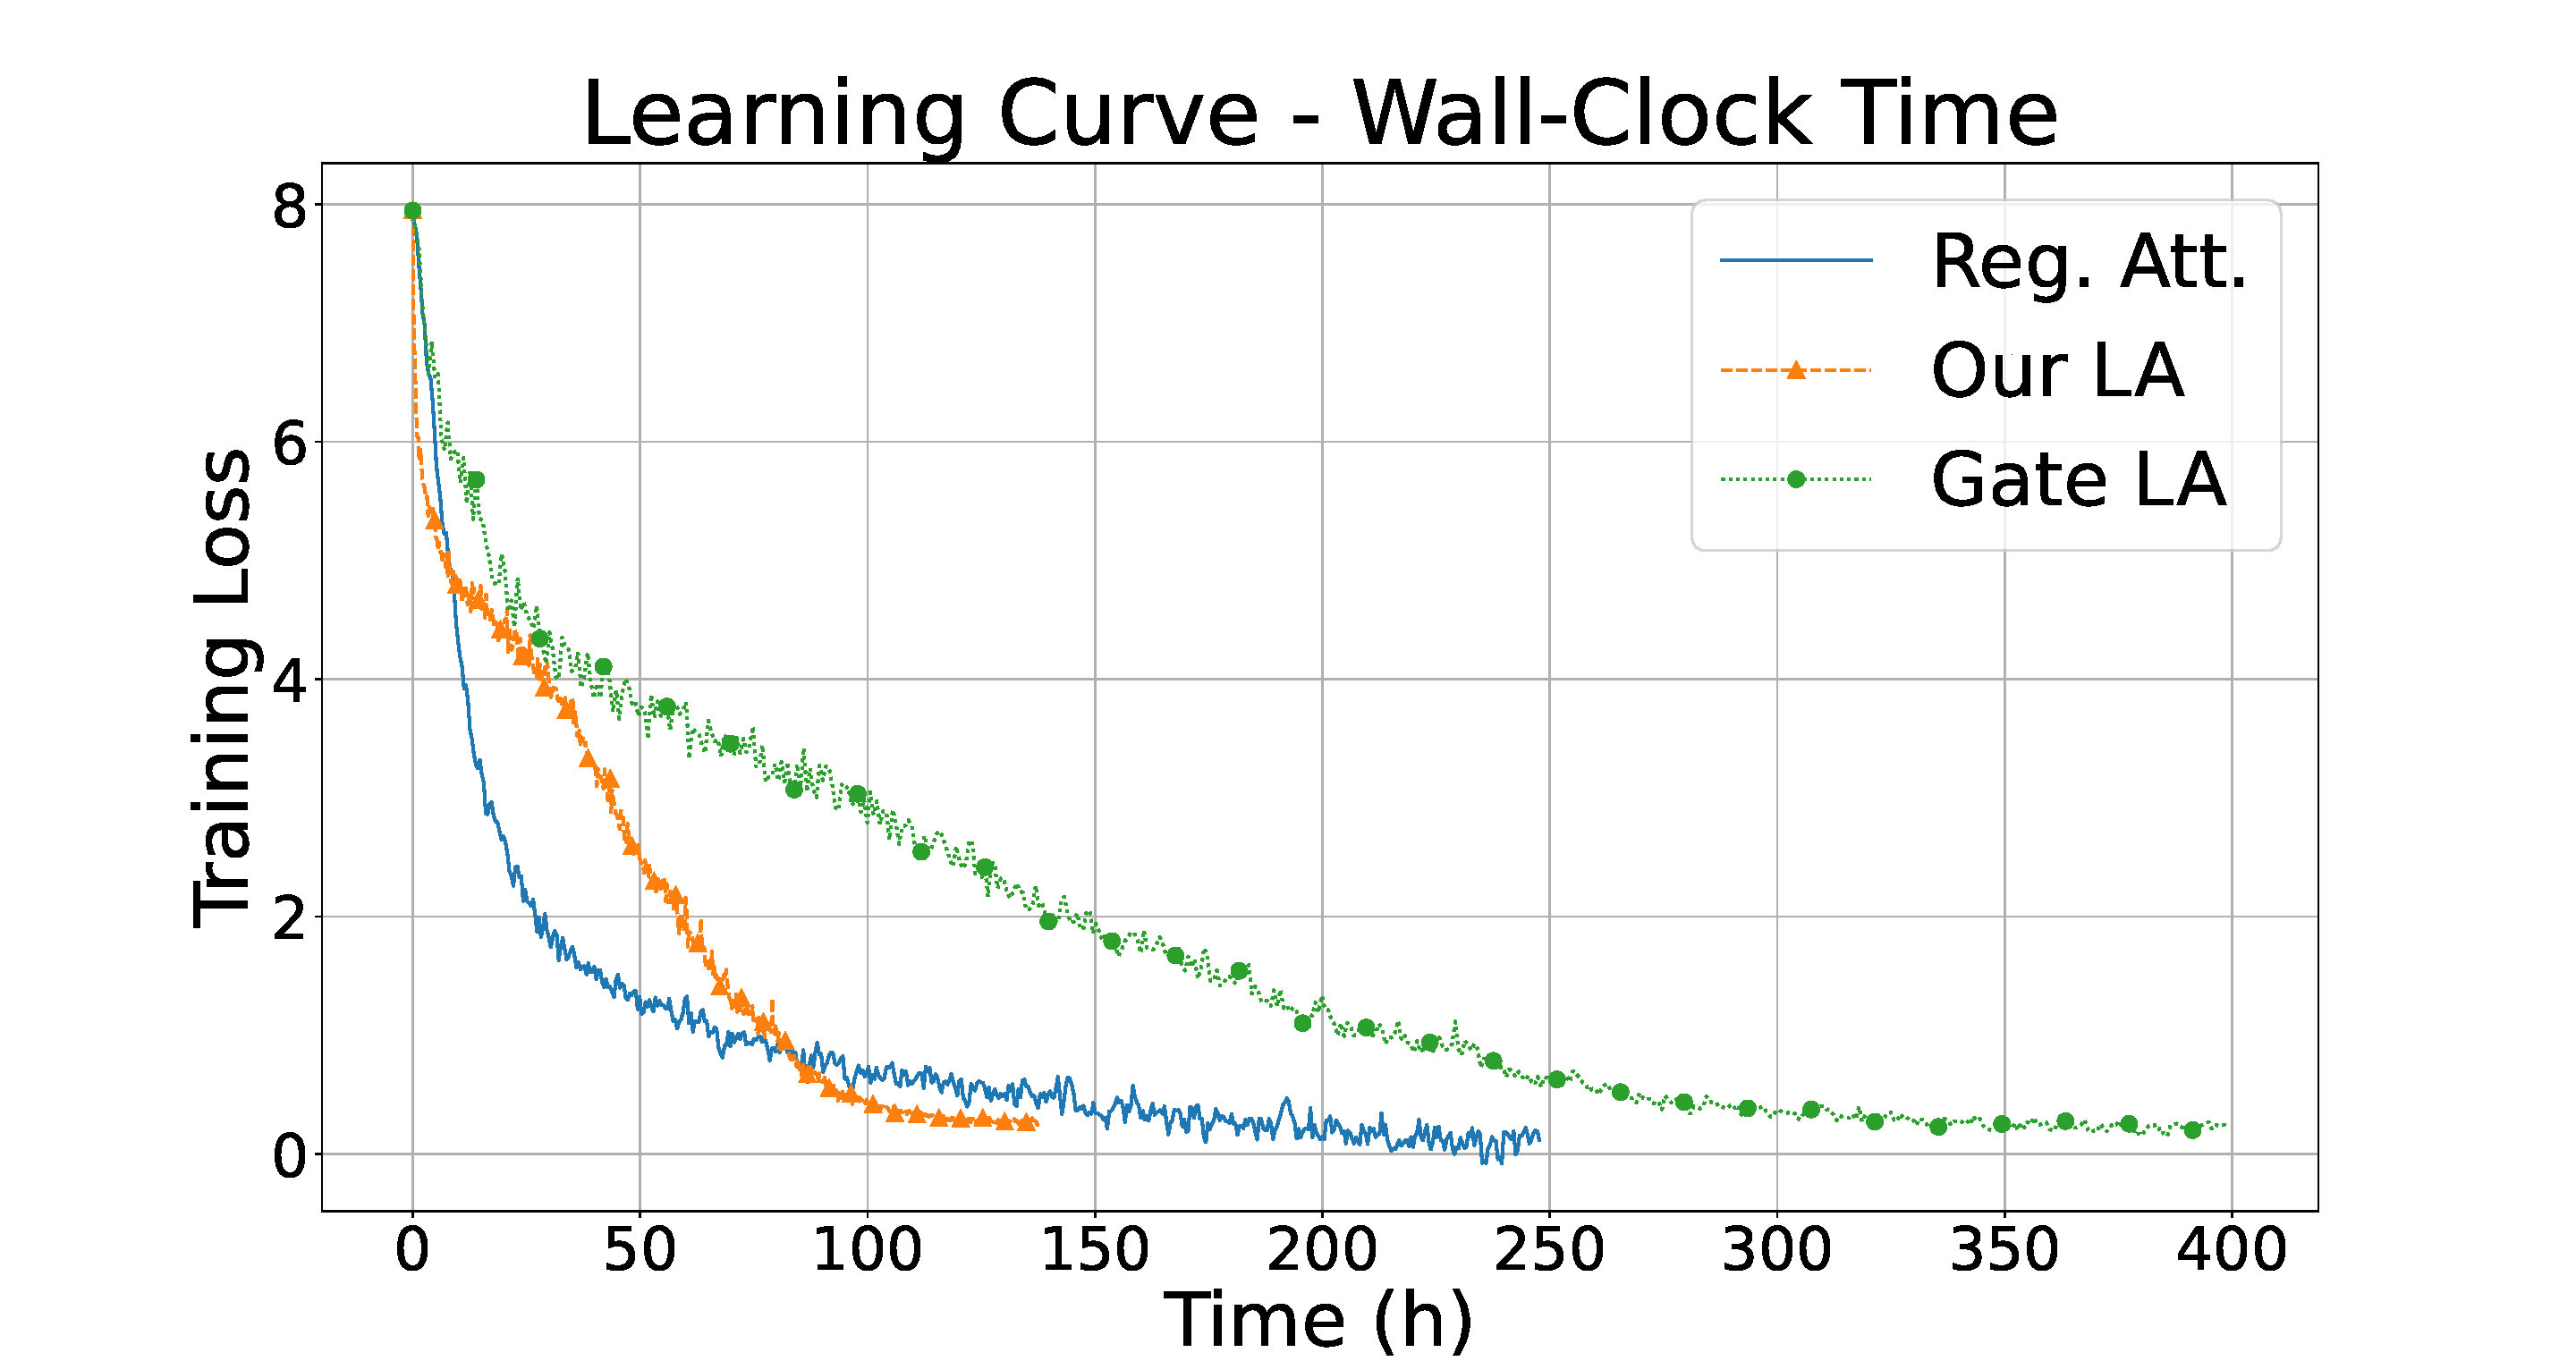
\includegraphics[width=0.49\linewidth, trim=28mm 0mm 40mm 30mm, clip=true]{images/learning_curve2.pdf} 
  % \hspace{0pt}\textbf{Learning Curve - Training Step}\par\medskip
  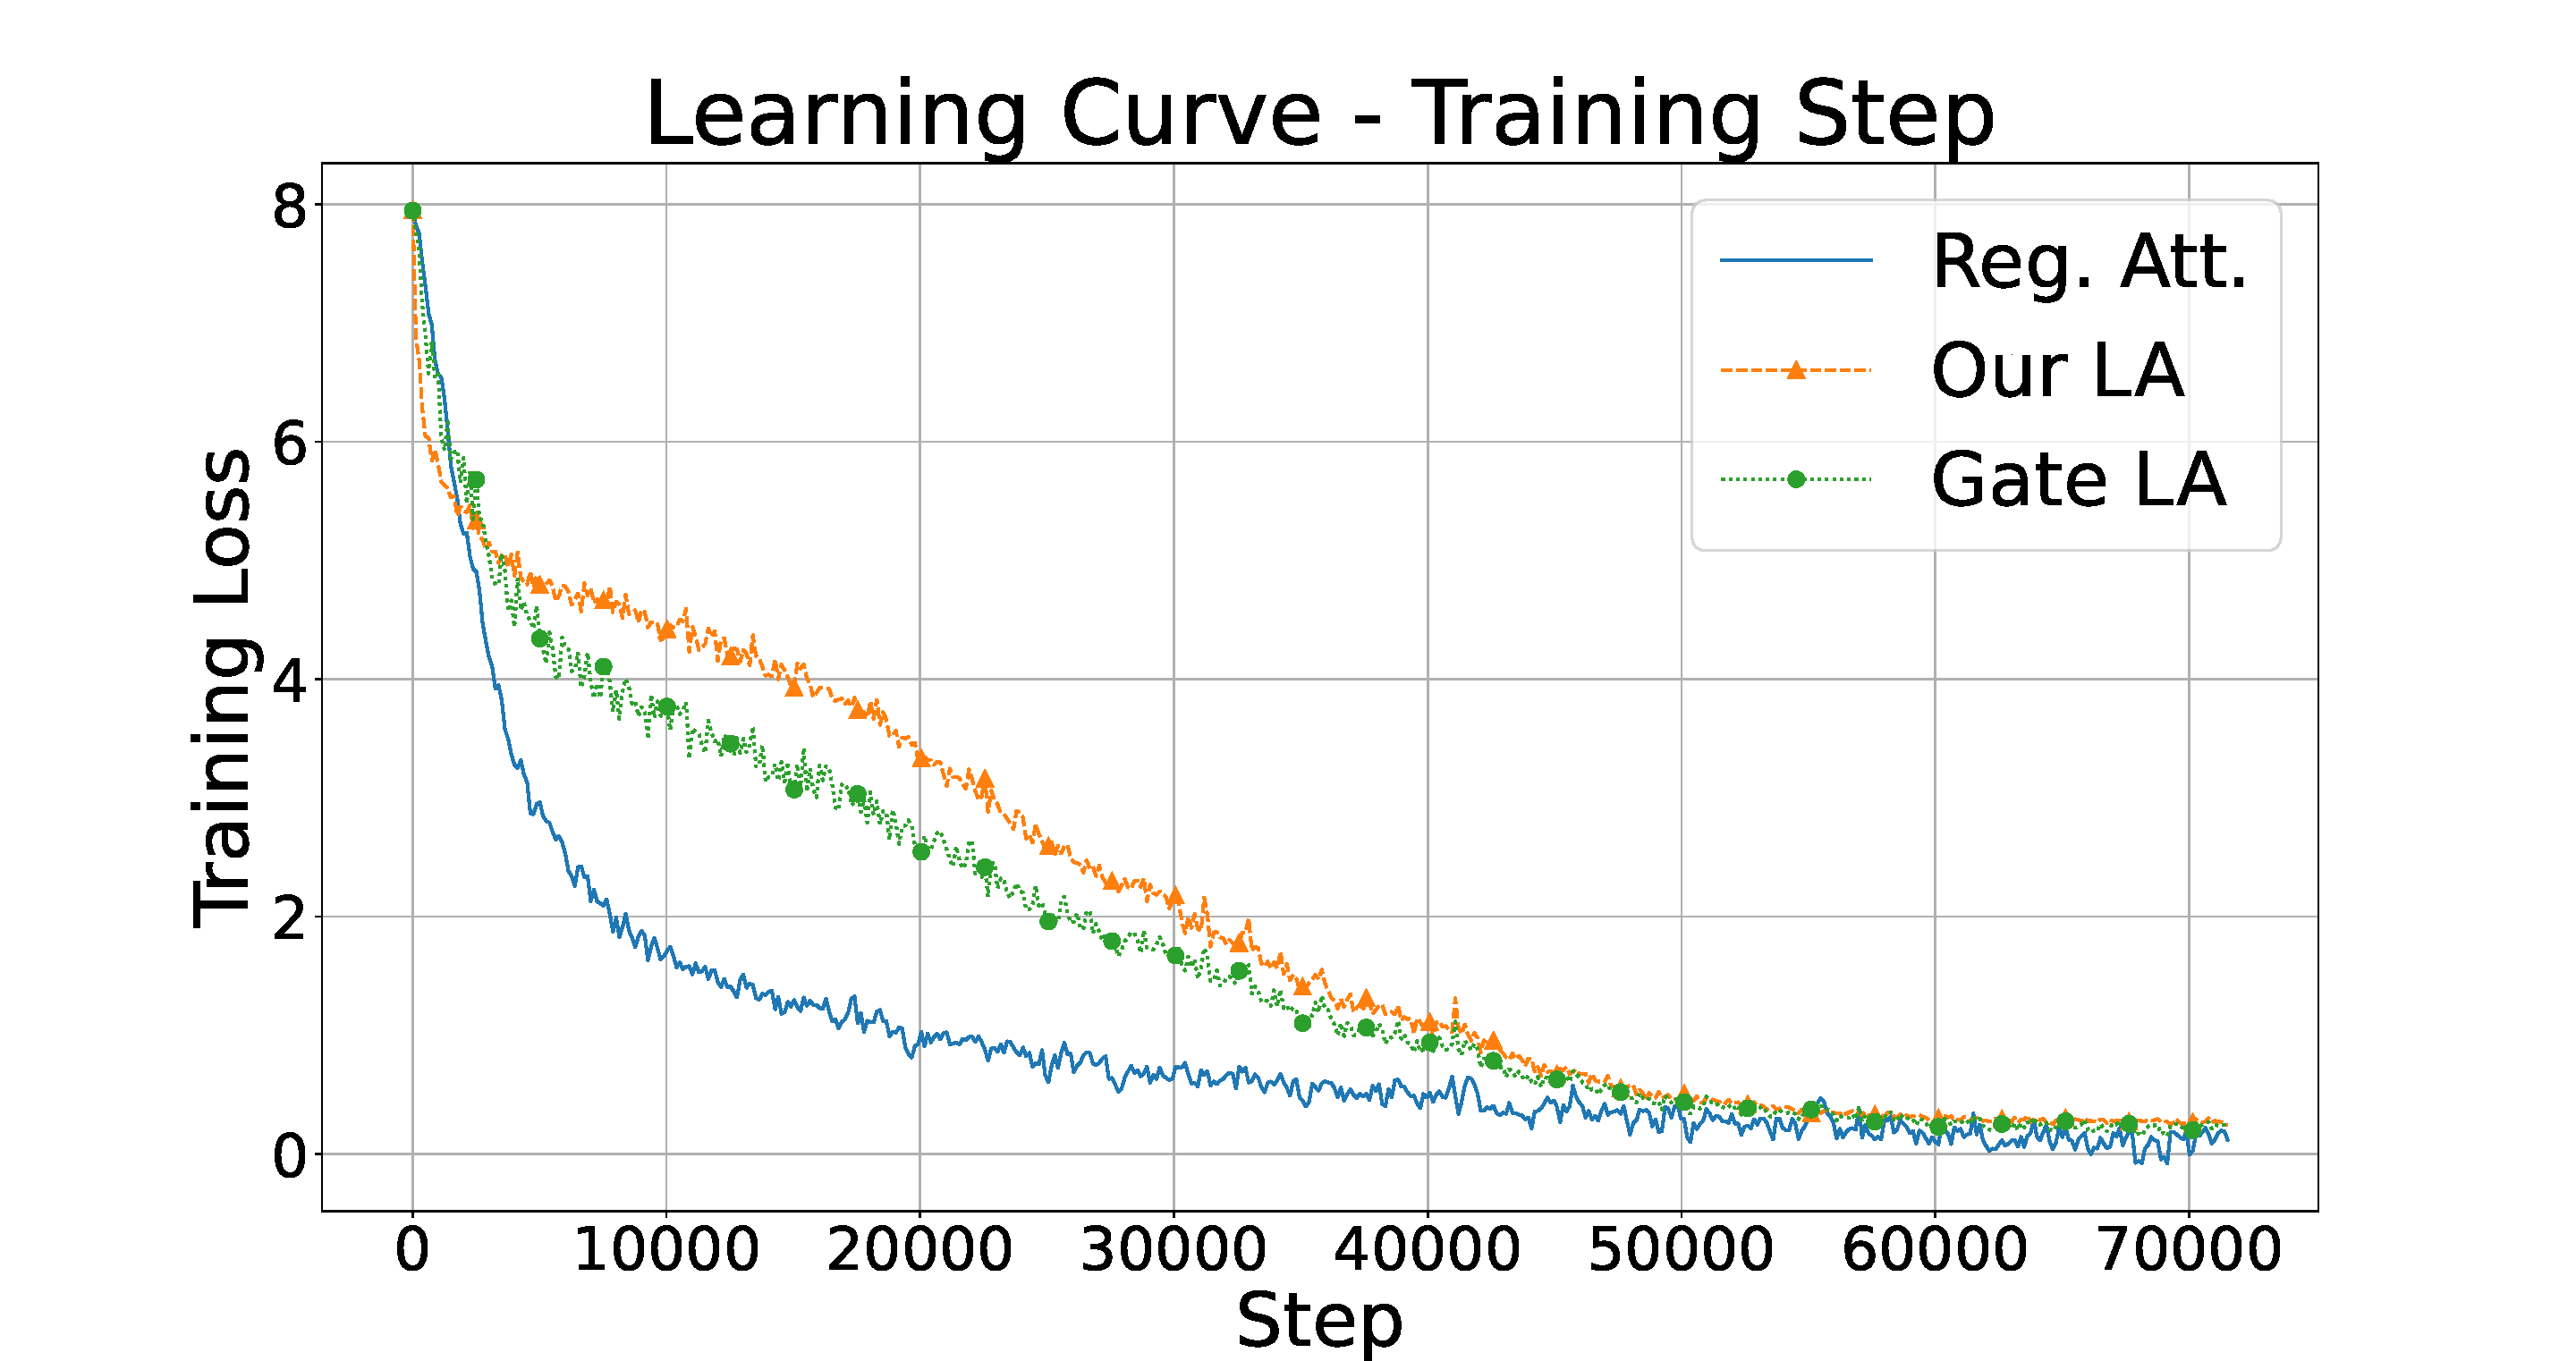
\includegraphics[width=0.49\linewidth, trim=28mm 0mm 40mm 30mm, clip=true]{images/learning_curve1.pdf}
  \caption{The learning curves of Pythia-1.4B, trained on the English segment of the Wiki-40B with a context length of $8192$ using eight A6000 GPUs. The learning curves are presented as a function of wall-clock time (left) and training step (right). Both models were trained for the same number of steps. Our linear attention (LA) implementation offers speedup over Regular Attention and Gated LA. The loss measures cross-entropy.}
  \label{curve} % Optional: Label for referencing later in the document
\end{figure}

\par Table~\ref{mmlu} shows the comparison between LA implementations and Regular Attention in terms of accuracy on a the MMLU~\cite{mmlu}, PIQA~\cite{piqa}, and ARC~\cite{arc} benchmarks. In agreement to results demonstrated by previous work~\cite{yang2023gated,you2024linear,pmlr-v119-katharopoulos20a,han2023flatten, cai2022efficientvit, zhang2024hedgehog, wangLinformerSelfAttentionLinear2020, shen2021efficient,arora2024simple}, LA is able to achieve comparable results to Regular Attention. This is significant as it implies that LA holds promise for replacing Regular Attention in resource-constrained devices such as smartphones, laptops, and edge devices. Our implementation of LA offers a substantial speedup over both state-of-the art LA implementation and efficient I/O aware Regular Attention in an end to end LLM setting, facilitating practical usage of LA.


\begin{table}[!h]
\caption{Comparing accuracy of Regular Attention and linear attention (LA) implementations. Unlike regular attention, which scales at $O(N^2)$ with the number of tokens $N$, LA scales linearly at $O(N)$ while achieving comparable accuracy.}
\vspace{-5pt}
\begin{center}
\resizebox{1\linewidth}{!}{
\begin{tabular}{l|ccccccccc}
\toprule
\textbf{Mechanism}&\makecell{\textbf{MMLU}\\(0-shot)}&\makecell{\textbf{MMLU}\\(5-shot)} & \textbf{PIQA} & \textbf{ARC-C}& \textbf{ARC-E}& \textbf{ARC-E}\\
\hline
Regular Attention & 22.10&23.04& 69.18& 33.83& 61.12& 60.34\\
\hline
Gated LA~\cite{yang2023gated}&   21.15&22.27& 65.38& 30.52& 57.73& 58.12\\
\hline
\textbf{Our LA} &  21.16&25.90& 68.63& 32.43& 59.95& 59.08\\
\bottomrule
\end{tabular}
}
\label{mmlu}
\end{center}
% \vspace{-5pt}
% \begin{tablenotes}
% \small
% \item \hspace{150pt} * The values reported are based on \cite{you2024linear}.
% \end{tablenotes}
\end{table}

% \begin{table}[!h]
% \caption{Comparing accuracy of Regular Attention and linear attention (LA) implementations. Unlike regular attention, which scales at $O(N^2)$ with the number of tokens $N$, LA scales linearly at $O(N)$ while achieving comparable accuracy.}
% \vspace{-5pt}
% \begin{center}
% \resizebox{1\linewidth}{!}{
% \begin{tabular}{l|ccccccc}
% \toprule
% \textbf{Mechanism}&\makecell{\textbf{MMLU}} & \textbf{PIQA} & \textbf{ARC-C}& \textbf{ARC-E}\\
% \hline
% Regular Attention & 23.04& 69.18& 33.83& 61.12\\
% \hline
% Gated LA~\cite{yang2023gated}&   22.27& 65.38& 30.52& 57.73\\
% \hline
% \textbf{Our LA} &  25.90& 68.63& 32.43& 59.95\\
% \bottomrule
% \end{tabular}
% }
% \label{mmlu}
% \end{center}
% % \vspace{-5pt}
% % \begin{tablenotes}
% % \small
% % \item \hspace{150pt} * The values reported are based on \cite{you2024linear}.
% % \end{tablenotes}
% \end{table}


